% ------------------------------------------------------------------------------
% Formatvorlage für Masterarbeiten an der Ohm-Hochschule Nürnberg
% ------------------------------------------------------------------------------
%   erstellt von Stefan Macke, 24.04.2009
%   http://blog.stefan-macke.de

% Dokumentenkopf ---------------------------------------------------------------
%   Diese Vorlage basiert auf "scrreprt" aus dem koma-script.
% ------------------------------------------------------------------------------
\documentclass[
    11pt, % Schriftgröße
    DIV=11,
    ngerman, % für Umlaute, Silbentrennung etc.
    a4paper, % Papierformat
    oneside, % einseitiges Dokument
    titlepage, % es wird eine Titelseite verwendet
    parskip=half, % Abstand zwischen Abstüzen (halbe Zeile)
    headings=normal, % Größe der Überschriften verkleinern
    listof=totoc, % Verzeichnisse im Inhaltsverzeichnis aufführen
    bibliography=totoc, % Literaturverzeichnis im Inhaltsverzeichnis aufführen
    bibliographyWebverzeichnis=totoc,
    index=totoc, % Index im Inhaltsverzeichnis aufführen
    captions=tableheading, % Beschriftung von Tabellen unterhalb ausgeben
    final % Status des Dokuments (final/draft)
]{scrreprt}

% Meta-Informationen -----------------------------------------------------------
%   Informationen über das Dokument, wie z.B. Titel, Autor, Matrikelnr. etc
%   werden in der Datei Meta.tex definiert und können danach global
%   verwendet werden.
% ------------------------------------------------------------------------------
% Meta-Informationen -----------------------------------------------------------
%   Definition von globalen Parametern, die im gesamten Dokument verwendet
%   werden k�nnen (z.B auf dem Deckblatt etc.).
%
%   ACHTUNG: Wenn die Texte Umlaute oder ein Esszet enthalten, muss der folgende
%            Befehl bereits an dieser Stelle aktiviert werden:
%            \usepackage[latin1]{inputenc}
% ------------------------------------------------------------------------------
\newcommand{\titel}{Implementierung und Bewertung eines Konzeptes zur "Content
					  Relevance-Oriented Data Transport (CRODT)"}
\newcommand{\untertitel}{und hier kommt der Untertitel}
\newcommand{\art}{Projektarbeit}
\newcommand{\fachgebiet}{Software-Engineering}
\newcommand{\autor}{Marian Haescher, Florian Ludwig, Philip Grunert}
\newcommand{\studienbereich}{}
\newcommand{\matrikelnrFLORIAN}{12 34 56}
\newcommand{\matrikelnrMARIAN}{12 34 56}
\newcommand{\matrikelnrPHILIP}{7200626}
\newcommand{\erstgutachter}{Prof. Dr. Werner Berentzen}
\newcommand{\zweitgutachter}{Dipl.-Inf. Lukas Podolski}
\newcommand{\jahr}{2012}
\newcommand{\ort}{Rostock}
\newcommand{\logo}{Bilder/unirostock_logo.jpeg}


% benötigte Packages -----------------------------------------------------------
%   LaTeX-Packages, die benötigt werden, sind in die Datei Packages.tex
%   "ausgelagert", um diese Vorlage möglichst übersichtlich zu halten.
% ------------------------------------------------------------------------------
% Anpassung des Seitenlayouts --------------------------------------------------
%   siehe Seitenstil.tex
% ------------------------------------------------------------------------------
\usepackage[
    automark, % Kapitelangaben in Kopfzeile automatisch erstellen
    headsepline, % Trennlinie unter Kopfzeile
    ilines % Trennlinie linksb�ndig ausrichten
]{scrpage2}

% Anpassung an Landessprache ---------------------------------------------------
\usepackage[ngerman]{babel}

% Umlaute ----------------------------------------------------------------------
%   Umlaute/Sonderzeichen wie ���� direkt im Quelltext verwenden (CodePage).
%   Erlaubt automatische Trennung von Worten mit Umlauten.
% ------------------------------------------------------------------------------
\usepackage[utf8]{inputenc}
%\usepackage[T1]{fontenc}
\usepackage{textcomp} % Euro-Zeichen etc.

% Schrift ----------------------------------------------------------------------
\usepackage{lmodern} % bessere Fonts
\usepackage{relsize} % Schriftgr��e relativ festlegen

% Grafiken ---------------------------------------------------------------------
% Einbinden von JPG-Grafiken erm�glichen
\usepackage[pdftex]{graphicx}
% hier liegen die Bilder des Dokuments
\graphicspath{{Bilder/}}

% Befehle aus AMSTeX f�r mathematische Symbole z.B. \boldsymbol \mathbb --------
\usepackage{amsmath,amsfonts}

% f�r Index-Ausgabe mit \printindex --------------------------------------------
\usepackage{makeidx}

% Einfache Definition der Zeilenabst�nde und Seitenr�nder etc. -----------------
\usepackage{setspace}
\usepackage{geometry}

% Symbolverzeichnis ------------------------------------------------------------
%   Symbolverzeichnisse bequem erstellen. Beruht auf MakeIndex:
%     makeindex.exe %Name%.nlo -s nomencl.ist -o %Name%.nls
%   erzeugt dann das Verzeichnis. Dieser Befehl kann z.B. im TeXnicCenter
%   als Postprozessor eingetragen werden, damit er nicht st�ndig manuell
%   ausgef�hrt werden muss.
%   Die Definitionen sind ausgegliedert in die Datei "Glossar.tex".
% ------------------------------------------------------------------------------
\usepackage[intoc]{nomencl}
\let\abbrev\nomenclature
\renewcommand{\nomname}{Abkürzungsverzeichnis}
\setlength{\nomlabelwidth}{.25\hsize}
\renewcommand{\nomlabel}[1]{#1 \dotfill}
\setlength{\nomitemsep}{-\parsep}

% zum Umflie�en von Bildern ----------------------------------------------------
\usepackage{floatflt}


% zum Einbinden von Programmcode -----------------------------------------------
\usepackage{listings}
\usepackage{xcolor} 
\definecolor{hellgelb}{rgb}{1,1,0.9}
\definecolor{colKeys}{rgb}{0,0,1}
\definecolor{colIdentifier}{rgb}{0,0,0}
\definecolor{colComments}{rgb}{1,0,0}
\definecolor{colString}{rgb}{0,0.5,0}
\lstset{
    float=hbp,
    basicstyle=\ttfamily\color{black}\small\smaller,
    identifierstyle=\color{colIdentifier},
    keywordstyle=\color{colKeys},
    stringstyle=\color{colString},
    commentstyle=\color{colComments},
    columns=flexible,
    tabsize=2,
    frame=single,
    extendedchars=true,
    showspaces=false,
    showstringspaces=false,
    numbers=left,
    numberstyle=\tiny,
    breaklines=true,
    backgroundcolor=\color{hellgelb},
    breakautoindent=true
}
\lstset{literate=%
{Ö}{{\"O}}1
{Ä}{{\"A}}1
{Ü}{{\"U}}1
{ß}{{\ss}}2
{ü}{{\"u}}1
{ä}{{\"a}}1
{ö}{{\"o}}1
}

% URL verlinken, lange URLs umbrechen etc. -------------------------------------
\usepackage{url}

% wichtig f�r korrekte Zitierweise ---------------------------------------------
\usepackage[square]{natbib}

% PDF-Optionen -----------------------------------------------------------------
\usepackage[
    bookmarks,
    bookmarksopen=true,
    colorlinks=true,
% diese Farbdefinitionen zeichnen Links im PDF farblich aus
    linkcolor=red, % einfache interne Verkn�pfungen
    anchorcolor=black,% Ankertext
    citecolor=blue, % Verweise auf Literaturverzeichniseintr�ge im Text
    filecolor=magenta, % Verkn�pfungen, die lokale Dateien �ffnen
    menucolor=red, % Acrobat-Men�punkte
    urlcolor=cyan, 
% diese Farbdefinitionen sollten f�r den Druck verwendet werden (alles schwarz)
    %linkcolor=black, % einfache interne Verkn�pfungen
    %anchorcolor=black, % Ankertext
    %citecolor=black, % Verweise auf Literaturverzeichniseintr�ge im Text
    %filecolor=black, % Verkn�pfungen, die lokale Dateien �ffnen
    %menucolor=black, % Acrobat-Men�punkte
    %urlcolor=black, 
    backref,
    plainpages=false, % zur korrekten Erstellung der Bookmarks
    pdfpagelabels, % zur korrekten Erstellung der Bookmarks
    hypertexnames=false, % zur korrekten Erstellung der Bookmarks
    linktocpage % Seitenzahlen anstatt Text im Inhaltsverzeichnis verlinken
]{hyperref}
% Befehle, die Umlaute ausgeben, f�hren zu Fehlern, wenn sie hyperref als Optionen �bergeben werden
\hypersetup{
    pdftitle={\titel \untertitel},
    pdfauthor={\autor},
    pdfcreator={\autor},
    pdfsubject={\titel \untertitel},
    pdfkeywords={\titel \untertitel},
}

% fortlaufendes Durchnummerieren der Fu�noten ----------------------------------
\usepackage{chngcntr}

% f�r (lange) Tabellen ---------------------------------------------------------
\usepackage{longtable}
\usepackage{array}
\usepackage{ragged2e}
\usepackage{lscape}
\usepackage{tabularx}

% Spaltendefinition rechtsb�ndig mit definierter Breite ------------------------
\newcolumntype{w}[1]{>{\raggedleft\hspace{0pt}}p{#1}}

% Formatierung von Listen �ndern -----------------------------------------------
\usepackage{paralist}

% bei der Definition eigener Befehle ben�tigt
\usepackage{ifthen}

% definiert u.a. die Befehle \todo und \listoftodos
\usepackage{todonotes}

% sorgt daf�r, dass Leerzeichen hinter parameterlosen Makros nicht als Makroendezeichen interpretiert werden
\usepackage{xspace}

% Erstellung eines Index und Abkürzungsverzeichnisses aktivieren ---------------
\makeindex
%\makenomenclature

% Kopf- und Fußzeilen, Seitenränder etc. ---------------------------------------
% Zeilenabstand 1,5 Zeilen -----------------------------------------------------
\onehalfspacing

% Seitenraender
% -----------------------------------------------------------------
\setlength{\topskip}{\ht\strutbox} % behebt Warnung von geometry
%\geometry{paper=a4paper,left=35mm,right=35mm,top=30mm} % Ohne Binderand


% Mit Binderand
%\geometry{a4paper,inner=3.5cm,outer=2.5cm,top=2.5cm,bottom=2.5cm,pdftex} 

\geometry{a4paper,inner=3.5cm,outer=2.5cm,top=2.5cm,bottom=2.5cm,pdftex} % Mit Binderand

% Kopf- und Fußzeilen ----------------------------------------------------------
\pagestyle{fancy} %scrheadings
% Kopf- und Fußzeile auch auf Kapitelanfangsseiten

\renewcommand*{\chapterpagestyle}{fancy}

% Schriftform der Kopfzeile und Fu�zeile

\fancyhead[ER]{\nouppercase{\sc\leftmark}}
\fancyhead[EL]{\nouppercase{\sc\rightmark}}
\fancyhead[OR]{\nouppercase{\sc\rightmark}}
\fancyhead[OL]{\nouppercase{\sc\leftmark}}

\fancyfoot[OL]{\copyright\ \autor}
\fancyfoot[OR]{\thepage}
\fancyfoot[EL]{\thepage}
\fancyfoot[ER]{\copyright\ \autor}
\fancyfoot[C]{}

% sonstige typographische Einstellungen ----------------------------------------

% erzeugt ein wenig mehr Platz hinter einem Punkt
\frenchspacing 

% Schusterjungen und Hurenkinder vermeiden
\clubpenalty = 10000
\widowpenalty = 10000 
\displaywidowpenalty = 10000

% Quellcode-Ausgabe formatieren
\lstset{numbers=left, numberstyle=\tiny, numbersep=5pt, breaklines=true}
\lstset{emph={square}, emphstyle=\color{red}, emph={[2]root,base}, emphstyle={[2]\color{blue}}}

% Fußnoten fortlaufend durchnummerieren
\counterwithout{footnote}{chapter}


% eigene Definitionen für Silbentrennung
\include{config/Silbentrennung}

% eigene LaTeX-Befehle
\include{config/Befehle}

% ------------ glossar initialisieren -----
%Ein eigenes Symbolverzeichnis erstellen
\newglossary[slg]{symbolslist}{syi}{syg}{Symbolverzeichnis} 

%Den Punkt am Ende jeder Beschreibung deaktivieren
\renewcommand*{\glspostdescription}{}

%Glossar-Befehle anschalten
\makeglossaries
%Befehle für Abkürzungen
\newacronym{DOID}{DOID}{Data Object Idendification Number}
\newacronym{FIFO}{FIFO}{First In First Out}
\newacronym{IF}{IF}{Interface}
\newacronym{STL}{STL}{Standard Template Library}
\newacronym{CRODM}{CRODM}{Content Relevance-oriented Data
 Management}
\newacronym{CROP}{CROP}{Content Relevance-Ortiented Protocol}
\newacronym{TCP}{TCP}{Transmission Control Protocol}
\newacronym{UDP}{UDP}{User Datagram Protocol}
\newacronym{DTN}{DTN}{Delay Tolerant Networks}
\newacronym{IPN}{IPN}{Interplanitary Internet}
\newacronym{CCSDS}{CCSDS}{Consultative Committee for Space Data Systems}
\newacronym{CFDP}{CFDP}{CCSDS File Delivery Protocol}
\newacronym{LTP}{LTP}{Licklider Transmission Protocol}
\newacronym{DSN}{DSN}{Deep Space Network}
\newacronym{TTL}{TTL}{Time To Live}
\newacronym{ASCII}{ASCII}{American Standard Code for Information Interchange}
\newacronym{IP}{IP}{Internet Protocol}
\newacronym{XML}{XML}{Extensible Markup Language}
\newacronym{CRODT}{CRODT}{Content Relevance-Oriented Data Transport}
\newacronym{GUI}{GUI}{Graphical User Interface}

%Befehle für Glossar
\newglossaryentry{glos:Packetizer}{
name=Packetizer,
description={packetizer noch hinzufügen}
}

\newglossaryentry{glos:Overlay}{
name=Overlay,
description={Overlay noch hinzufügen}
}

% Befehle für Symbole
% \newglossaryentry{symb:Pi}{
% name=$\pi$,
% description={Die Kreiszahl.},
% sort=symbolpi, type=symbolslist
% }
% \newglossaryentry{symb:Phi}{
% name=$\varphi$,
% description={Ein beliebiger Winkel.},
% sort=symbolphi, type=symbolslist
% }
% \newglossaryentry{symb:Lambda}{
% name=$\lambda$,
% description={Eine beliebige Zahl, mit der der nachfolgende Ausdruck
% multipliziert wird.},
% sort=symbollambda, type=symbolslist
% }


% beispiel einer Abkürzung mit Glossareintrag
% \newacronym{AD}{AD}{Active Directory\protect\glsadd{glos:AD}}
% \newglossaryentry{glos:AntwD}{
% name=Antwortdatei,
% description={Informationen zum
% Installieren einer Anwendung oder des Betriebssystems.}
% }


% Das eigentliche Dokument -----------------------------------------------------
%   Der eigentliche Inhalt des Dokuments beginnt hier. Die einzelnen Seiten
%   und Kapitel werden in eigene Dateien ausgelagert und hier nur inkludiert.
% ------------------------------------------------------------------------------
\begin{document}

% auch subsubsection nummerieren
\setcounter{secnumdepth}{3}
\setcounter{tocdepth}{3}

% Deckblatt und Abstract ohne Seitenzahl
\ofoot{}
%!TEX root = ./Literaturarbeit.tex
\begin{titlepage}
		\begin{center}
		
			\begin{figure}[H]
				\centering
				\includegraphics[scale=.3]{Bilder/unirostock_logo.jpeg}
			\end{figure}
			\textbf{\large Universität Rostock\\}
			\vspace{1.5cm}
			\textbf{\large Fakultät für Informatik und Elektrotechnik\\}
			\vspace{0.2cm}
			\textbf{\large Institut für Automatisierungstechnik\\}
			\vspace{1.5cm}
			\textbf{\Large Bachelorarbeit\\}
			\vspace{1.5cm}
			\textbf{\large ``Modellbasierte Optimierung von Stellgrößentrajektorien\\}
			\vspace{0.2cm}
			\textbf{\large  in zyklisch arbeitenden Herzunterstützungssystemen unter\\}
			\vspace{0.2cm}
			\textbf{\large medizinischen und technischen Randbedingungen"\\}
			\vspace{3cm}
			
			\textbf{\centering
			\begin{tabularx}{400pt}{ll}
				Bearbeiter: & Philip Grunert\\
				Studiengang: & ITTI\\
				Matrikelnummer: & 7200626\\
				Bearbeitungszeitraum: & 01.06.2011 - 07.09.2011\\
				Betreuender Hochschullehrer: & Prof. Dr.-Ing. habil. Dr. h.c. Bernhard Lampe \\ 
				Betreuer: & M.Sc. Alexander Sievert \\
			\end{tabularx}
			}		
				
		\end{center}	
	\end{titlepage} 

% Aufgabenstellung
\thispagestyle{empty}
\includepdf[pages=-]{Aufgabenstellung.pdf}
\ofoot{\pagemark}
% Seitennummerierung -----------------------------------------------------------
%   Vor dem Hauptteil werden die Seiten in großen römischen Ziffern 
%   nummeriert.
% ------------------------------------------------------------------------------
\pagenumbering{Roman}
\tableofcontents % Inhaltsverzeichnis

% Abkürzungsverzeichnis
% --------------------------------------------------------
% % für eine korrekte Überschrift in der Kopfzeile
\clearpage %\markboth{\nomname}{\nomname}
 %\printnomenclature 
\printindex
% \label{sec:Glossar}
 
%\cleardoublepage{}
 
%Glossar ausgeben
\printglossary[style=altlist,title=Glossar]
 
%Abkürzungen ausgeben
\deftranslation[to=German]{Acronyms}{Abkürzungsverzeichnis}
\printglossary[type=\acronymtype,style=long]

%Symbole ausgeben
\printglossary[type=symbolslist,style=long]
 

\listoffigures % Abbildungsverzeichnis
\listoftables % Tabellenverzeichnis
\renewcommand{\lstlistlistingname}{Verzeichnis der Listings}
\lstlistoflistings % Listings-Verzeichnis

% arabische Seitenzahlen im Hauptteil ------------------------------------------
\clearpage
\pagenumbering{arabic}

% die Inhaltskapitel werden in "Inhalt.tex" inkludiert -------------------------
\chapter{Einleitung}
	Seit {\"u}ber f{\"u}nfzig Jahren entwickeln Forscher Strategien
zur Erkundung des Weltraums. Dabei hat sich seit der Entsendung des ersten k{\"u}nstlichen
Satelliten namens Sputnik und der ersten Mondlandung viel getan.
Zahlreiche Sonden oder Landefahrzeuge wurden seither zu diversen Zielen unseres
Sonnensystems entsandt, um neue Erkenntnisse {\"u}ber unser Universum und dessen
Entstehung zu sammeln. Ein aktuelles Beispiel stellt der Mars Rover Curiosity
dar, welcher j{\"u}ngst im Gale Krater auf dem Mars landete. Der Rover
verf{\"u}gt {\"u}ber zahlreiche Messinstrumente, darunter Kameras, Sensoren zur
Messung kosmischer Strahlung, Spektrografen, meteorologische Messinstrumente und
vieles mehr. Der Rover selbst ist mit einem Gewicht von $900$ kg und der
Gr{\"o}{\ss}e eines kompakten Kleinwagens das bisher mit Abstand gr{\"o}{\ss}te
vom Menschen geschaffene Objekt, das je die Marsoberfl{\"a}che erreichte.
\textit{Curiosity} stellt ein mobiles Labor dar, das neben den Sensoren und
Messinstrumenten auch Greifarme und R{\"a}der zur Fortbewegung und Interaktion
aufweist. Alle Messinstrumente und s{\"a}mtliche Peripherie des Rovers werden dabei von der
Erde aus gesteuert. Mit steigender Komplexit{\"a}t der mobilen Labore
steigt nat{\"u}rlich auch die Menge an Daten, die es zu {\"u}bertragen gilt. Da
die komplette Steuerung und Auswertung auf der Erde stattfindet, gilt es, sowohl
Steuerdaten von der Erde an den Rover zu senden, als auch Messdaten, Bilder und
{\"a}hnliches vom Rover an die Erde zu {\"u}bermitteln. Dabei unterliegt die
Kommunikation einigen entscheidenden Restriktionen. Die wohl Wichtigste ist die
Lichtgeschwindigkeit, welche sich im Vakuum mit $299 792 458$ m/s ausbreitet.
Die Ausbreitung der entsandten Signale kann daher niemals schneller erfolgen. Da die
Entfernung zum Mars je nach Konstellation variiert, ist es im Folgenden
hilfreich, von der mittleren minimalen Entfernung zur Erde auszugehen. Diese
betr{\"a}gt $0,52$ AE oder aber ca. $77,8$ Millionen Kilometer (Schwankung des
$[Erde - Mars]$ Abstandes je nach Konstellation: $0,372 - 2,683$ AE, d.h. bei
Opposition $[Sonne - Erde - Mars]$ zwischen ca. $55 - 105$ Millionen Kilometern
und bei Konjunktion $[Mars - Sonne - Erde]$ ca. $400$ Millionen Kilometer).
Ausgehend von dieser Entfernung, bei einer Ausbreitungsgeschwindigkeit der
Signale von ca. $300.000$ km/s, erh{\"a}lt man eine Dauer von ca. $4,3$ Minuten
pro {\"U}bertragungsrichtung. Daraus folgt, dass die Antwort, auf eine an den
Mars gesandte Anfrage bei diesem Szenario im Idealfall nach $8,6$
Minuten, die Erde erreicht (im Fall der maximalen Entfernung zwischen Erde und
Mars erst nach $44$ Minuten, wobei in dieser Konstellation eine direkte
Funkverbindung nahezu unm{\"o}glich ist).
Da der Mars jedoch genau wie die Erde eine Rotation um seine eigene Achse
ausf{\"u}hrt und die Kommunikation {\"u}ber eine den Mars
umkreisende Sendevorrichtung (Satellit) erfolgt, wird das Zeitfenster der
{\"U}bertragung weiter beschr{\"a}nkt (Zeitfenster betr{\"a}gt ca. 30 Minuten
pro Tag aufgeteilt in zwei Sendevorg{\"a}nge von je 15 Minuten, dies ist jeweils
die Zeit f{\"u}r den Vorbeiflug des Orbiters von Horizont zu Horizont bezogen
auf den Rover).
Diese physikalisch begr{\"u}ndeten Latenzen sind ein wichtiger Faktor, den es in
der interplanetaren Kommunikation zu ber{\"u}cksichtigen gilt. Die hieraus
abzuleitende Erkenntnis ist, dass eine Kommunikation beispielsweise zwischen
Erde und Mars nicht mit einer heutigen irdischen Kommunikation zu vergleichen
ist. Zwar ist das Modell der verz{\"o}gerten Kommunikation dem Menschen
keineswegs unbekannt.
Hier sei Exemplarisch auf den vor der Erfindung der Telegraphie
ausschlie{\ss}lich betriebenen Briefverkehr verwiesen. Jedoch ist dieses
Ph{\"a}nomen in der heutigen vernetzten Generation nahezu in Vergessenheit
geraten. Die irdische Kommunikation im $21$. Jahrhundert setzt auf geringe
Latenzen und kann somit idealisiert als verz{\"o}gerungsfrei betrachtet werden.
Doch eine interplanetare Kommunikation wird nicht allein durch die
unvermeidlichen Latenzen beeinflusst. Auch die Bandbreite unserer
{\"U}bertragung unterliegt der Erde abgewandten Seite einer Beschr{\"a}nkung. Am
Beispiel der Mars Rover sei hier auf die genutzten Solarpanele bzw. eingesetzten
Batterien (zumeist Radionuklidbatterien) verwiesen, welche nur eine begrenzte
Energieversorgung gew{\"a}hrleisten und somit keine nahezu unbegrenzte
Sendeleistung erm{\"o}glichen, wie es auf der Erde der Fall ist.
Ein weiterer Punkt ist die f{\"u}r den Rover eingesetzte Technologie. Hierbei 
sind unter anderem Faktoren wie Gr{\"o}{\ss}e und Gewicht von Bedeutung, da 
diese die Kosten der Unternehmung stark beeinflussen. So kostet beispielsweise 
der Start einer Ariane $5$ Rakete zwischen $125$ und $155$ Millionen Euro bei 
einer Nutzlast von $23.000$ kg im LEO (Low Earth Orbit: $200-2.000$ km).
Hieraus ergibt sich f{\"u}r dieses Beispiel ein Preis von ca. $7.000$ Euro pro kg 
Nutzlast. An diesem Beispiel zeigt sich die Wichtigkeit einer genauen
Kalkulation des Gewichtes der Rover. Diese Restriktion wirkt sich direkt auf die
verbaute Hardware des Rovers aus und somit auch indirekt auf Ressourcen wie z.B.
die Gr{\"o}{\ss}e des verbauten Speichers zum Ablegen lokaler Daten.
Zusammenfassend kann anhand der Beispiele festgestellt werden, dass Latenz, 
Bandbreite sowie lokaler Speicher wichtige Restriktionen sind, denen die 
interplanetare Kommunikation unterliegt. Diese Voraussetzungen verlangen 
eine besondere Kommunikationsstruktur die von den {\"u}blichen Protokollen 
abweicht. Das \gls{CROP} soll hier f{\"u}r Abhilfe sorgen.
Der Gedanke des Protokolls ist ein gezielter Umgang mit den begrenzten 
Ressourcen. Hierbei wird einerseits eine Verallgemeinerung der vorhandenen 
Daten in Datenbl{\"o}cke vorgenommen und andererseits eine Priorisierung der 
Daten erwirkt, welche {\"u}ber die Reihenfolge und den Zeitpunkt des 
Versendens entscheidet. Daraus resultiert, dass Daten von hoher Relevanz 
vor Daten mit niederer Relevanz verschickt werden. Somit k{\"o}nnen 
beispielsweise zeitkritische Daten das Kontrollzentrum auf der Erde 
schneller erreichen. Im Folgenden wird ein kurzer {\"U}berblick zu den einzelnen
Kapiteln der Arbeit gew{\"a}hrt.

In \textbf{Kapitel zwei} werden die Grundlagen der Netzwerkkommunikation
aufgef{\"u}hrt, welche zum Verst{\"a}ndnis der Arbeit notwendig sind. Dabei wird
\zB das OSI-Referenzmodell aufgegriffen und erl{\"a}utert. Die im Weiteren
erl{\"a}uterten Modelle k{\"o}nnen alle vom OSI-Schichtenmodell abgeleitet
werden. Die weiteren Grundlagen betreffen die Zeitmessung auf dem Mars und
andere allgemeine Erl{\"a}uterungen.

Das \textbf{dritte Kapitel} befasst sich mit dem aktuellen Stand der Technik.
Hier werden aktuelle Technologien und Protokolle vorgestellt, welche in der
interplanetaren Kommunikation zum Einsatz kommen.

\textbf{Kapitel vier} umfasst das Konzept der Arbeit. Hier werden
Vor{\"u}berlegungen ausgef{\"u}hrt und grundlegende Funktionen erl{\"a}utert.
Zudem werden einige Ideen beleuchtet, welche in der weiteren
Protokollentwicklung zu ber{\"u}cksichtigen sind, die aber im derzeitigen Stand
nicht implementiert wurden.

\textbf{Kapitel f{\"u}nf} behandelt die Implementierung des Protokolls. Dabei
wird sowohl die Implementierung der betreffenden Module für das Protokoll
genauer beleuchtet, als auch die Entwicklung der grafischen Benutzeroberfläche
f{\"u}r eine einfache Chat Kommunikation.

Im \textbf{sechsten Kapitel} wird die ausf{\"u}hrliche Analyse des Protokolls
betrachtet.
Dabei wird eine Overhead- sowie eine Speicherverbrauch- und
Laufzeitanalyse diskutiert.

Im \textbf{siebten und letzten Kapitel} wird eine Zusammenfassung und ein
Ausblick auf die zuk{\"u}nftige Entwicklung im bearbeiteten Themenbereich gegeben.



\chapter{Grundlagen}
	Diese Kapitel befasst sich mit den Grundlagen die zum Verst{\"a}ndnis der Arbeit
notwendig sind. Dies umfasst allgemeine Grundlagen im Bereich der
Netzwerktechnik sowie Themen von Wichtigkeit f{\"u}r eine Interplanetare Kommunikation.

	\section{Protocol Stack}
		Der Protocol Stack bzw. Protokollstapel bezeichnet die Verschachtelung der
einzelnen Schichten die zur Erf{\"u}llung einer Protokollkommunikation
notwendig sind. Dabei werden die Daten der vorherigen Schicht genommen und zur
Weiterverarbeitung der nachfolgenden Schicht zugef{\"u}hrt. Dieses Stapelprinzip
gibt dem Protocol Stack seinen Namen. Der Stack {\"u}bernimmt dabei
s{\"a}mtliche Koordination und Verarbeitung der Datenstr{\"o}me (z.B.
Segmentierungen, Adressierung etc.).
Je nach Anforderung an die Kommunikation muss der Stack angepasst werden. Die
eingehenden Daten werden dann im Top-Ddown-Verfahren durch den Stack verpackt
und einer Sendqueue zugef{\"u}hrt nach dem Versenden werden sie auf der
Empfangsseite im Bottom-Up-Verfahren wieder ausgepackt und k{\"o}nnen
anschließend ausgewertet werden.

	\section{OSI-Modell}
		Das OSI-Modell besteht aus sieben Schichten und ist eine allgemeine Beschreibung
bzw. Designrichtlinie f{\"u}r Kommunikationsprotokolle (siehe Abb.
\ref{fig:OSI_M}).

\begin{figure}[H]
\centering
\includegraphics[scale=.3]{OSI_M.pdf}
\caption{Das OSI-Referenzmodell}
\label{fig:OSI_M}
\end{figure}

\textbf{Physical Layer}

Der Physical Layer stellt eine physische Verbindung {\"u}ber das jeweilige
Medium her (z.B. Kupferkabel, Wireless etc.). Hier findet die eigentliche
Bit{\"u}bertragung statt.

\textbf{Data Link Layer}

Der Data Link Layer soll eine sichere {\"U}bertragung gew{\"a}rleisten. Diesem
obliegt somit das Herstellen einer Ende-zu-Ende Verbindung (Link), um eine
{\"U}bertragung zu erm{\"o}glichen. Dazu geh{\"o}rt die Einteilung der Daten in
Frames, das hinzuf{\"u}gen von Pr{\"u}fsummen sowie die Kanalkodierung und eine
Datenflusskontrolle (Protokollbeispiele: Ethernet, FDDI).

\textbf{Network Layer}

Der Network Layer sorgt f{\"u}r die Weitervermittlung von Datenpaketen. Der
Schicht obliegt die Adressierung von Datenpaketen (via IP) und das Routing
(Aufbau von Routingtabellen etc.). Protokollbeispiele in dieser Schicht: IP, ICMP.

\textbf{Transport Layer}

Die Aufgaben des Transport Layer sind die Segmentierung des Datenstroms sowie
Stauvermeidung und Bereitstellung von Felersicherungs- und
Fehlerbehebungsverfahren (Protokollbeispiele: TCP, UDP).

\textbf{Session Layer}

Zu den Aufgaben des Session Layer geh{\"o}ren die Handhabung von
Verbindungsabbr{\"u}chen und das daraus resultierende Setzen von
Sicherungspunkte (Checkpoints). Diese erm{\"o}glichen eine Wiederaufnahme
nach einem erfolgten Abbruch. Somit wird eine st{\"a}ndige Synchronit{\"a}t der
Dienste gew{\"a}rleistet (Protokollbeispiele: HTTP, FTP).

\textbf{Presentation Layer}

Der Presentation Layer erm{\"o}glicht eine Darstellung von Daten in
einer unabh{\"a}ngigen Form (dies garantiert eien Datenaustausch zwischen
unterschiedlichen Systemen). Desweiteren werden die Daten hier Komprimiert und
Verschl{\"u}sselt (Protokollbeispiele: HTTP, FTP).

\textbf{Application Layer}

Der Application Layer verwaltet den Zugriff der Anwendung auf das Netzwerk
(Protokollbeispiele: HTTP, FTP).

	\section{CROP}
		Das \gls{CROP} bezeichnet einen Protokoll-Stack, der zur relevanzabh{\"a}ngigen
Daten{\"u}bertragung in \gls{DTN} eingesetzt wird. Dabei
umfasst das daf{\"u}r entwickelte Framework sowohl das Splitten von beliebigen
Daten, als auch eine Evaluierung selbiger. Die Evaluierung geschieht entweder
automatisch (z.B. mit einer Ontologie), oder manuell durch die menschlichen
Kommunikationspartner, die unter Nutzung von CROP miteinander kommunizieren
\cite{Daher}.

	\section{Zeitmessung}
		\label{sec:zeitmessung}

Durch die unterschiedlichen Umlaufzeiten der Planeten um die Sonne wird eine
Umrechnung der Zeit auf der Erde zu der Zeit auf dem Mars ben{\"o}tigt.
Dadurch k{\"o}nnen auf dem Mars aufgenommene Daten eindeutig zugeordnet
werden.
F{\"u}r diese Berechnung wird das heliozentrische Weltbild (die Erde dreht sich
um die Sonne) genutzt, wodurch die Sonne zum gemeinsamen Bezugspunkt f{\"u}r
Erde und Mars wird.

Die Erde bewegt sich mit einer Geschwindigkeit von $27 km/s$ auf einer
elliptischen aber fast kreisf{\"o}rmigen Umlaufbahn um die Sonne (siehe Bild
\ref{fig:marsEarthOrbit}).

\begin{figure}[H]
	\centering
	\includegraphics[scale=.5]{earthmarsorbittop.pdf}
	\caption[Umlaufbahn von Erde und Mars]{Umlaufbahn von Erde und Mars \cite{img1}}
	\label{fig:marsEarthOrbit}
\end{figure}

Die Drehrichtung ist rechtl{\"a}ufig. Das hei{\ss}t, die Bewegung erfolgt
entgegen dem Uhrzeigersinn um die Sonne. Mit gleichem Drehsinn erfolgt eine Eigenrotation
der Erde. Diese wird als sidierischer Tag bezeichnet und ist nach $23$ Stunden
und $56$ Minuten vollzogen. Die fehlenden $4$ Minuten zu dem uns gel{\"a}ufigen
$24$ Stunden-Tag (Sonnentag) lassen sich durch {\"a}u{\ss}ere Einwirkungen,
wie die Anziehungskraft der Sonne, erkl{\"a}ren. Von dieser Betrachtung
ausgehend, ben{\"o}tigt die Erde f{\"u}r einen einmaligen Umlauf um die Sonne
$365.2424$ Sonnentage, was einem Erdenjahr (tropisches Jahr) oder einem
terrianischen Jahr entspricht.

Die selben Voraussetzungen gelten f{\"u}r den Mars. Die Abbildung
\ref{fig:marsEarthOrbit} zeigt f{\"u}r den Mars eine elliptischere Bahn
auf. Dies hat eine Verschiebung der Tages- und Jahreszeiten zur Folge. Somit ist
auf dem Mars ein Sonnentag exakt $24$ Stunden, $39$ Minuten und $35.24$ Sekunden lang und
wird "`Sol"' (Sol, engl. solar day) genannt. Nach $686.9710$ Erd-Sonnentagen
bzw. $669$ Sol hat der Mars die Sonne einmal vollst{\"a}ndig umkreist. Um eine Beziehung
und somit eine Umrechnung der Zeiten zwischen Planeten vorzunehmen, muss die
Einteilung der Monate und Jahreszeiten aus Sicht der Sonne vorgenommen werden.

Im Weiteren wird eine M{\"o}glichkeit zur Umrechnung der Erdzeit auf Marszeit
nach Robert Zubrin, vorgestellt welcher auch den Begriff "`Sol"'
f{\"u}r einen Marstag pr{\"a}gte. Die nachfolgende Abbildung zeigt den von Zubrin entwickelten
Marskalender (Abbildung \ref{fig:marsEarthCalendar} links) im Vergleich zu dem
bekannten gregorianischen Kalender. Die Monate sind hierbei zur einheitlichen
Bestimmung in Form der lat. Namen der Tierkreiszeichen benannt, welche zu jener
Zeit von der Sonne aus gesehen durchzogen werden.

\begin{figure}[H]
	\centering
	\includegraphics[width=\textwidth]{marsEarthCalendar.png}
	\caption[Kalender: Mars und Erde]{Kalender: Mars und Erde \cite{img2}}
	\label{fig:marsEarthCalendar}
\end{figure}

Bei der Umrechnung zwischen diesen beiden Kalendern bezog sich Zubrin auf das
Jahr $1965$. Dort fielen der Beginn des Erdenjahres ($1.$ Januar), sowie der
Beginn des Marsjahres ($1.$ Gemini) aufeinander. Daraus ergab sich der
nachfolgende Ansatz:

\begin{equation}
	Marsjahr \quad = \quad \frac{8}{15} \quad * \quad (Erdenjahr -
	1961) \quad + \quad 1
	\label{eq:marsYear}
\end{equation}

Das Erdenjahr folgt einer dezimalen Darstellung und setzt sich wie in Formel
\ref{eq:earthYear} zusammen. Zum Tragen kommen hierbei das aktuelle Jahr sowie
die numerischen Angaben von Tag ($numAktTag$) und Monat ($numAktMonat$) des
umzurechnenden Datums. Dies wird ins Verh{\"a}ltnis zur Gesamtanzahl der Tage in
einem Jahr gesetzt.

\begin{equation}
	Erdenjahr \quad = \quad aktuelleJahr + \frac{ (numAktMonat - 1) * 30.4 +
	(numAktTag - 1) }{365}
	\label{eq:earthYear}
\end{equation}

Diese soll am Beispiel der Marslandung des Rovers \textit{Curiosity} am
$6.$ August $2012$ verdeutlicht werden.

Aus Gleichung \ref{eq:earthYear} wird zun{\"a}chst das dezimale Erdenjahr
berechnet.
Es ergibt sich:

\begin{eqnarray}
	Erdenjahr \quad & = & \quad 2012 + \frac{ (8-1) * 30.4 + (6-1) }{365} \\
	Erdenjahr \quad & = & \quad 2012 + 0.59 \\
	Erdenjahr \quad & = & \quad 2012.59
\end{eqnarray}

und in die Gleichung \ref{eq:marsYear} eingesetzt

\begin{eqnarray}
	Marsjahr \quad & = & \quad \frac{8}{15} * (2012.59 - 1961) + 1 \\
	Marsjahr \quad & = & \quad 28.51
\end{eqnarray}

folgt das Marsjahr $28$. Der jeweilige Tag und Monat des Jahres wird
schlussendlich durch die Gleichung \ref{eq:MarsMonthSol} und die Tabelle
\ref{fig:marsEarthCalendar} bestimmt.

\begin{eqnarray}
	Marstag \quad & = & \quad \#MarstageImJahr * restMarsjahr \\
	Marstag \quad & = & \quad 666 * 0.51 \\
	Marstag \quad & = & \quad 340 Sol 
	\label{eq:MarsMonthSol}
\end{eqnarray}

Damit ist die Marssonde \textit{Curiosity} am $22.$ Sol im Sternbild Scorpius
des Marsjahres $28$ auf dem Mars gelandet.

Zubrin's Ansatz weist einige Fehler auf, die auf den ersten Blick keine
gr{\"o}{\ss}eren Probleme verursachen, aber auf weite Sicht starke
Verschiebungen der Zeiten zur Folge haben. Die Annahme, ein Erdenjahr sei immer $365$ Tage lang (siehe Formel
\ref{eq:earthYear}), kann nicht verallgemeinert werden. Vielmehr muss von einem
Mittel ausgegangen werden, da die L{\"a}nge eines Erdenjahres aufgrund der sich
wechselnden Abst{\"a}nde zur Sonne variiert. Hier wird das sogenannte Tropische Jahr
herangezogen, welches $365.2424$ Tage lang ist. Davon ausgehend ist eine
Korrektur des in der Formel \ref{eq:earthYear} angenommenen Verh{\"a}ltnisses von
Mars- zu Erdenjahr (erster Term) auf $\frac{7.97}{15}$ notwendig (Nachweis ab
Formel \ref{eq:errorKorrektur}).

\begin{eqnarray}
	\frac{MarsJahr}{ErdenJahr} \quad & = & \quad \frac{686.9710 \ Tage}{365.2424 \
	Tage}
	\\
	\label{eq:errorKorrektur}  
	\frac{MarsJahr}{ErdenJahr} \quad & = & \quad 1.88 \\
	\notag\\
	x \quad & = & \quad \frac{15}{1.88} \\
	x \quad & = & \quad 7.97 
\end{eqnarray}

Damit w{\"u}rde sich das Landungsdatum der Marssonde auf den $16.$ Sol im Sternbild
Libre verschieben. Nach nur knapp $50$ Jahren der Zeitrechnung Mars stellt sich
bereits eine Verschiebung von $66$ Sol (\ca 1 Marsmonat) ein. Dies zeigt, dass
eine exakte Umrechnung der Daten notwendig ist, um eine langfristige und exakte
Angabe {\"u}ber das Datum und die Zeit auf dem Mars machen zu k{\"o}nnen
\cite{web10}.

\section{Zusammenfassung des Kapitels}

Das in diesem Kapitel erkl{\"a}rte OSI-Schichtenmodell ist die Grundlage
s{\"a}mtlicher Kommunikationsprotokolle. Mit Hilfe dieses Modells besteht daher
im Weiteren die M{\"o}glichkeit, eine Einordnung bzw. einen Vergleichs der in
dieser Arbeit beschriebenen Protokolle vorzunehmen. Zudem wurde eine Auffrischung bzw.
grundlegende Einleitung in die wichtigste Terminologie der Netzwerktechnik
gegeben. Desweiteren wurde in diesem Kapitel eine detaillierte
Aufschl{\"u}sselung der Marszeitberechnung vorgenommen. Diese ist f{\"u}r
zuk{\"u}nftige Kommunikationsmodelle von gro{\ss}er Bedeutung, da hiermit eine
einheitliche und standardisierte Bezeichnung m{\"o}glich ist. Somit kann die
Bedeutungsgleichheit von Zeitsignalen im Austausch mit der Erde
gew{\"a}hrleistet werden. Diese Betrachtungen sollten vor allem unter
Ber{\"u}cksichtigung der Tatsache gesehen werden, dass Signale mit Zeitstempeln
versehen werden, die an Marsgegebenheiten angepasst werden m{\"u}ssen.
Dies resultiert aus der Tatsache, dass eine irdische Zeitrechnungen hier
schlichtweg nicht zutreffend sind.




\chapter{Stand der Technik}
  \label{cap:standDerTechnik}
Dieser Abschnitt befasst sich mit dem aktuellen Stand der Technik. Dies umfasst
sowohl die gegenw{\"a}rtig eingesetzte Hardware, als auch bereits
entwickelte Protokolle zur Interplanetaren Kommunikation.


\textbf{Mars Rover Curiosity}

Der Mars Rover Curiosity (Abb. \ref{fig:Curiosity}) verf{\"u}gt {\"u}ber einen
RAD750 Prozessor von BAE-Systems.
Dieser hat eine Taktfrequenz von bis zu 200 MHz und kann 266 MIPS oder mehr
verarbeiten. Desweiteren verf{\"u}gt Curiosity {\"u}ber einen Arbeitsspeicher von 256 MB
und einen Flash-Speicher von 2 GB. Zus{\"a}tzlich hat Curiosity einen EPROM von 256
KB. Alle Bauteile sind dabei besonders Strahlungsresistent und unempfindlich
gegen{\"u}ber gro{\ss}en Temperaturschwankungen. Das genutzte Betriebssystem ist
VxWorks. Zur Kommunikation nutzt der Rover
einerseits das X-Band (7 - 8 GHz), welches zur {\"U}bertragung von Statusdaten
und zum Empfang von Steuerdaten genutzt wird. Desweiteren verf{\"u}gt der Rover
{\"u}ber ein Kommunikationssystem im UHF-Band (0,4 GHz) welches f{\"u}
wissenschaftliche Daten mit hohem Datenvolumen genutzt wird (bis zu 250 Mbit
pro Tag, somit ca. 30 MB/Tag). Die Ausstattung an wissenschaftlichen
Instrumenten umfasst zehn Ger{\"a}te. Darunter z.B. zwei Mastkameras welche je
eine Aufl{\"o}sung von 1200 x 1200 Pixeln haben (1,44 Megapixel). Diese Kameras
sind ebenfalls in der Lage 720p-Videos mit einer Framerate von 10 Bildern pro
Sekunde aufzunehmen. Hinzu kommen Spektrografen, weitere Kameras, Sensoren etc.,
welche weitere Analysedaten beisteuern.

\begin{figure}[H]
\centering
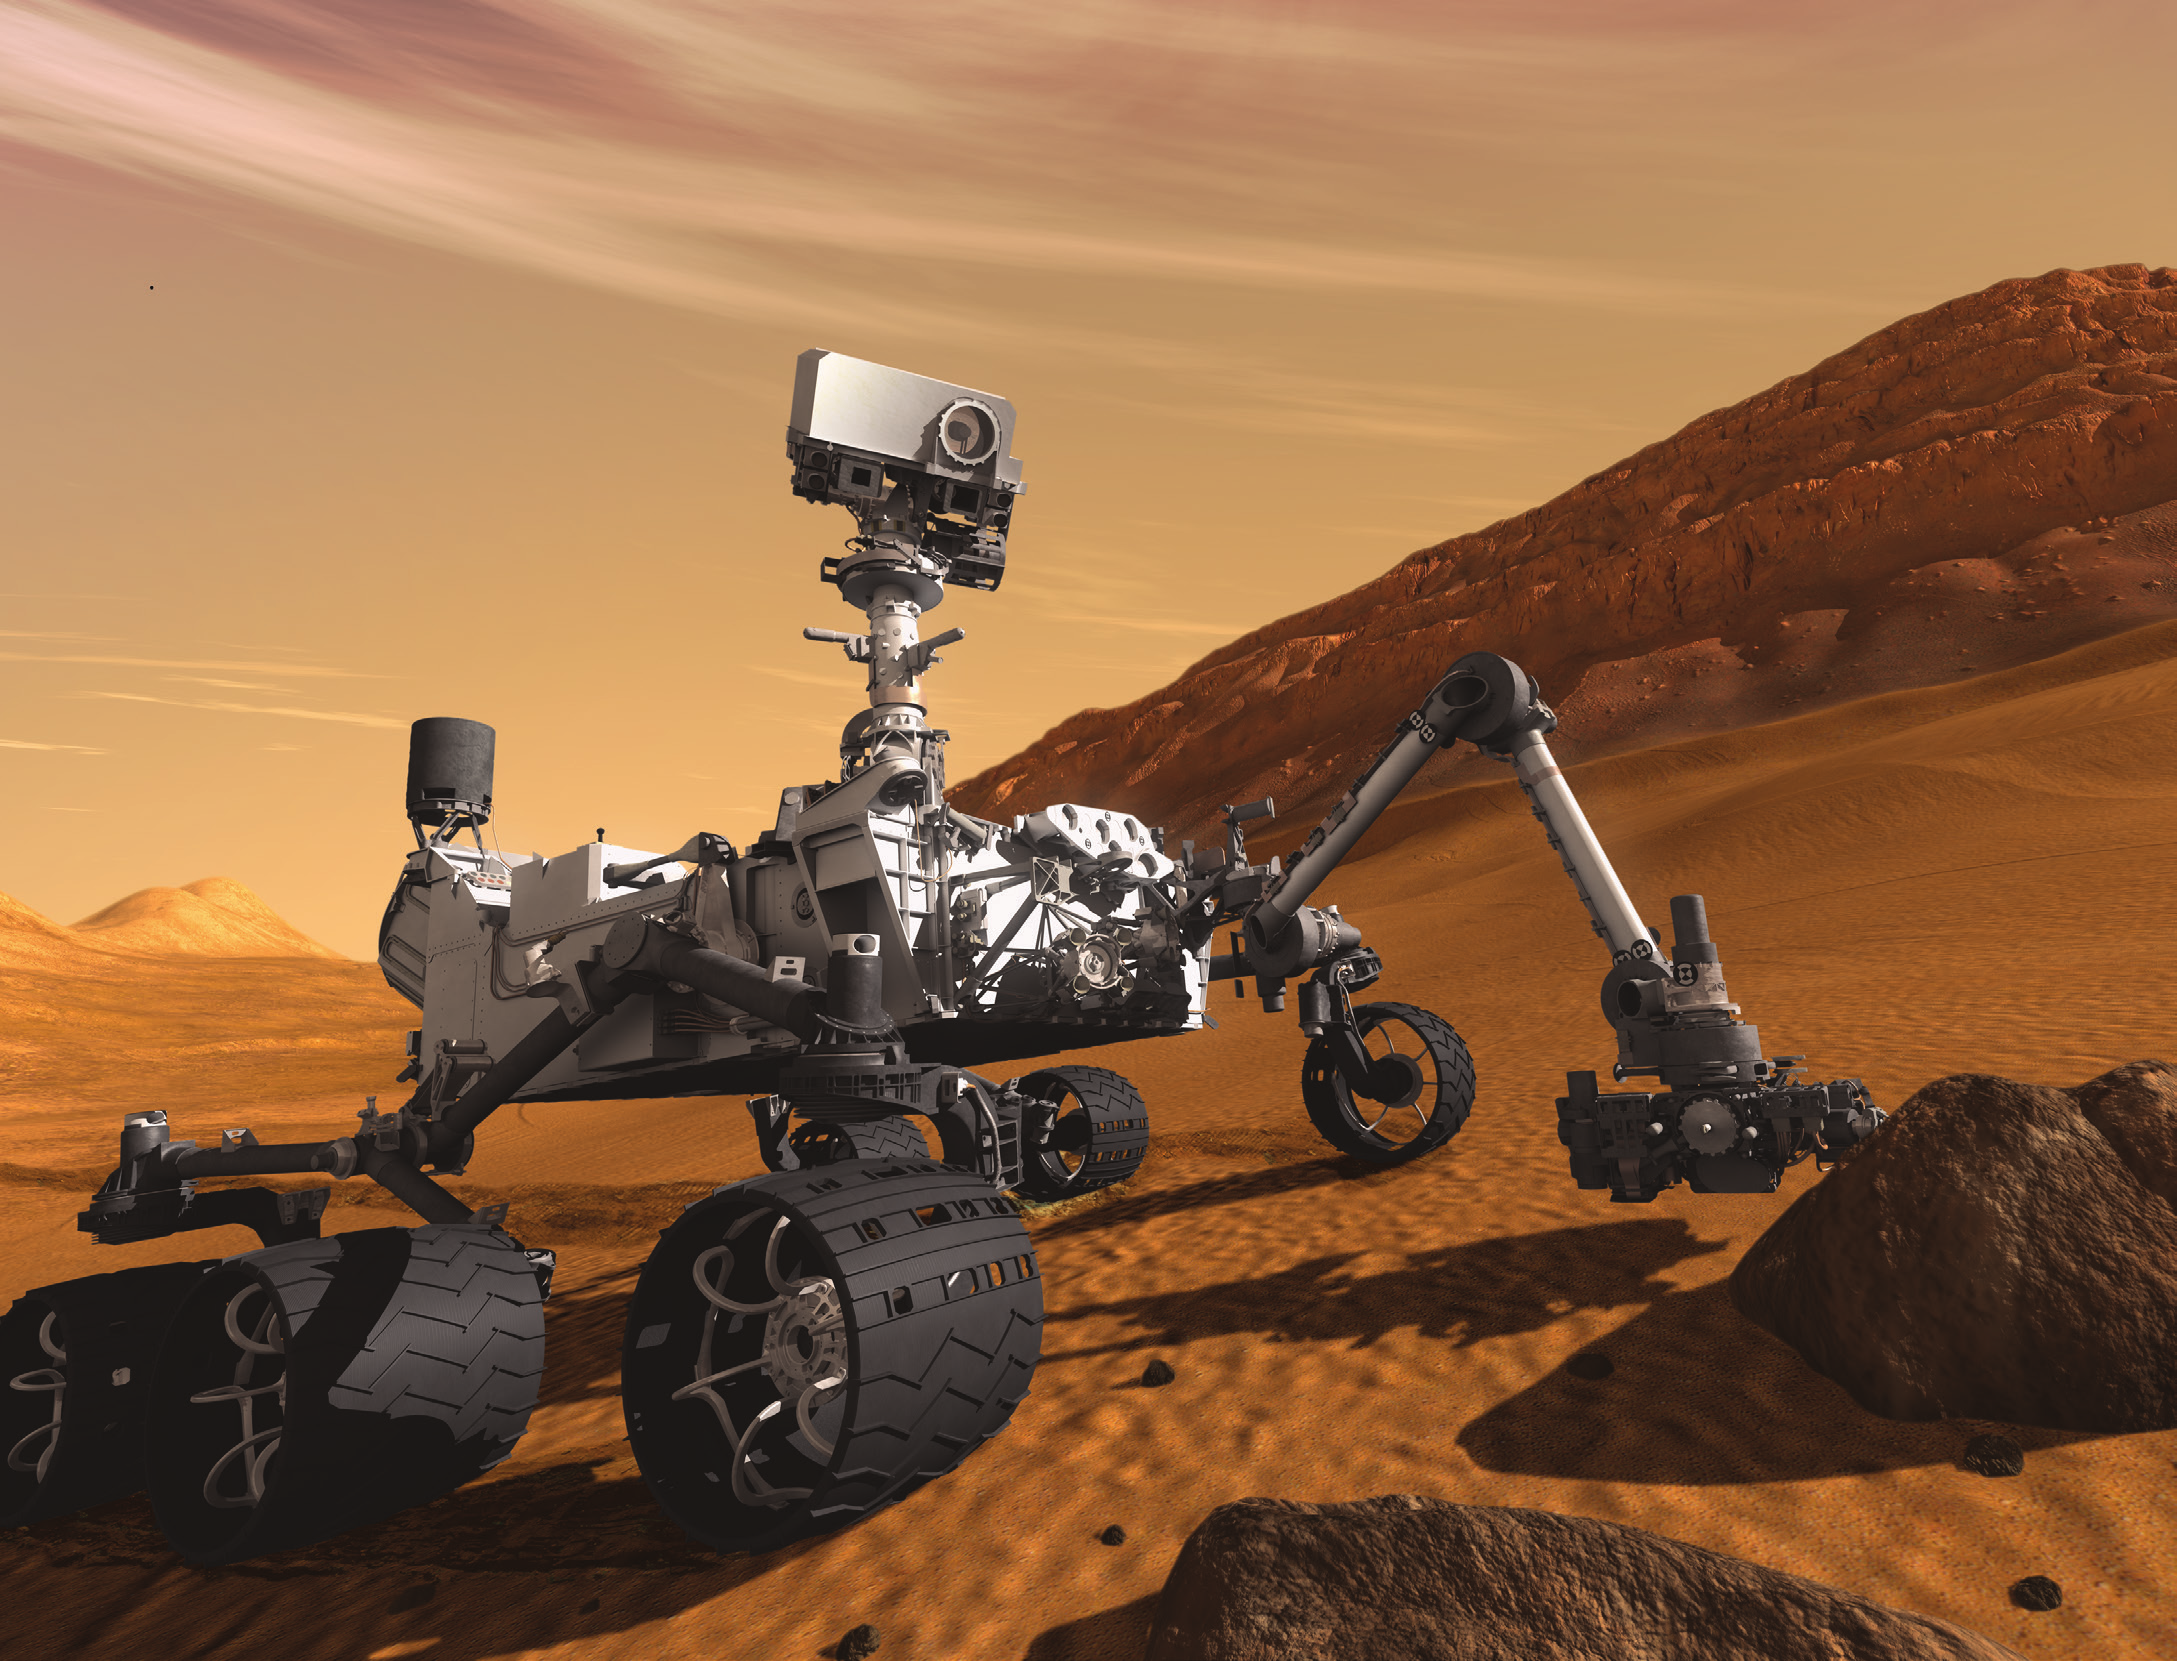
\includegraphics[scale=.09]{Curiosity.png}
\caption{Mars Rover Curiosity}
\label{fig:Curiosity}
\end{figure}

\textbf{Deep Space Network}

Das Deep Space Network bezeichnet ein Netz von Parabolantennen, welche zur
Kommunikation mit Raumsonden, Satelliten sowie radio-
und radarastronomischen Zwecken dienen. F{\"u}r die NASA werden derzeit die
folgenden drei gro{\ss}en Stationen betrieben:

\begin{compactenum}[a)]
\item \textit{Goldstone Deep Space Communication Complex, Kalifornien, USA
(Abb.} \ref{fig:Goldstone}\textit{)}
\item \textit{Madrid Deep Space Communication Complex, Madrid, Spanien}
\item \textit{Canberra Deep Space Communication Complex, Canberra, Australien}
\end{compactenum}

Das Deep Space Network wird auch f{\"u}r die Kommunikation zwischen dem Mars
Rover Curiosity und der Erde genutzt. Die Anlagen liegen an exponierter Position
(zumei{\ss}t h{\"u}geliges schalenf{\"o}rmiges Gel{\"a}nde). Dies soll den
Einfluss von St{\"o}rungen z.B. durch Radiofrequenzen reduzieren. Die Stationen
befinden sich je in einem Abstand von einem drittel Erd{\"a}quator um eine
fortw{\"a}hrende Kommunikation mit Raumfahrzeugen trotz Erdrotation zu
erm{\"o}glichen.

\begin{figure}[H]
\centering
\includegraphics[scale=.3]{Goldstone.jpg}
\caption{Antenne der NASA Deep Space Network Einrichtung in Goldstone,
Kalifornien, USA}
\label{fig:Goldstone}
\end{figure}

\textbf{Interplanitary Internet}

Das IPN bezeichnet die Erweiterung des Internets auf einen au{\ss}erirdischen
Bereich. Die damit verbundenen {\"A}nderungen im Vergleich zum Irdischen
Internet umfassern z.B. einen gesonderten Umgang mit Latenzen, da diese beim IPN
im Minuten bis Stunden Bereich liegen. Die Entwicklung von Protokollen
f{\"u}r das IPN obliegt dabei dem Consultative Committee for Space Data Systems
(CCSDS).

\textbf{Delay Tolerant Networking}

DTN bezeichnet eine Protokollarchitektur f{\"u}r End-to-end Netzwerkverbindungen
mit geringer stabilit{\"a}t. Die Basis der DTN Netzwerkarchitektur stellt das
von der NASA entwickelte IPN (Interplanitary Internet) dar. Ein wichtiger
Bestandteil dieser Netzwerke ist der Umgang mit gro{\ss}en Latenzen. zudem
m{\"u}ssen die an der Kommunikation beteiligten Knoten (Teilnehmer) Daten so
lange zwischen bis der Empf{\"a}nger den erhalt quittiert hat
(store-and-forward).

\textbf{Bundle-Protokoll}

Die in den RFCs 4838 und 5050 festgelegten Anforderungen f{\"u}r DTN sind
weitgehend unter der bezeichnung Bundle-Protokoll bekannt. In diesem werden Folgen von
Datenbl{\"o}cken als B{\"u}ndel zusammengefasst. Jedes B{\"u}ndel enth{\"a}lt
dabei ausreichende semantische Informationen um eine etwaige Applikation
fortzusetzen. Exemplarisch sei hier ein Webbrowser angef{\"u}hrt, welcher ein
Bundle-Paket erh{\"a}lt und dadurch eine Komplette Webseite anzeigt. Auch hier
erfolgt die {\"U}bertragung per store-and-forward. Die eingesetzten
Transportprotokolle k{\"o}nnen dabei variieren (IP basierend o.a.). Das
Bundle-Protokoll z{\"a}hlt zu den Overlay-Netzwerken, welche auf einer bereits
bestehenden Netzwerkstruktur aufsetzen.

\todo{Quellen und weitere ausf{\"u}hrungen zum bundle protokoll}

\textbf{Licklider Transmission Protocol}

Das LTP kann direkt auf dem Data Link Layer aufsetzen oder aber auch unter UDP
laufen (siehe Abb. \ref{fig:LTP}). LTP wird zudem als standard convergence layer
Protokoll f{\"u}r das Bundle Protokoll genutzt. Das LTP wurde zur sicheren {\"U}bertragung von Daten
zwischen einem Sender und einem Empf{\"a}nger (point-to-point) unter DTN Bedingungen entwickelt. LTP entscheidet dabei sogar zwischen wichtigen
(red data) und unwichtigen Daten (green data) und gew{\"a}hrleistet somit eine
effiziente {\"U}bermittlung. Eine {\"U}bertragung beginnt sobald ein Link zwischen Sender und Empf{\"a}nger
besteht. Die zu sendenden Datenbl{\"o}cke werden beim LTP in Segmente
geteilt. Handelt es sich um wichtige Daten (red data) so werden w{\"a}hrend des
Sendevorgangs innerhalb der im LTP verwendeten Segmente spezielle Flags gesetzt.
Diese einfach als Checkpoints bezeichneten Signale erfordern eine Quittierung durch den Empf{\"a}nger um so bei einem eventuellen
Verbindungsabbruchs eine erneute Sendung des jeweiligen Datenpakets
auszul{\"o}sen. Die Daten werden so lange beim Sender in einer Queue
vorgehalten, bis der zugeh{\"o}rige Checkpoint quittiert wurde. Wenn ein
Checkpoint nicht quittiert wird kann durch einen ablaufenden Timer auf seiten
des Senders ein erneutes Senden getriggert werden. Sowohl das Senden als auch
Empfangen eines Blocks kann per Signal abgebrochen werden. Zudem ist die
Gr{\"o}{\ss}e der Segmente einstellbar um sie an den jeweiligen zweck
anzupassen. Handelt es sich bei den zu Sendenden Daten um Daten geringerer
Relevanz (green data) so ist keine Best{\"a}tigung durch den Empf{\"a}nger
vonn{\"o}ten.
Diese Daten werden direkt nach dem Versenden gel{\"o}scht.

\begin{figure}[H]
\centering
\includegraphics[scale=.5]{LTP.pdf}
\caption{Eiordnung des LTP in das Kommunikationsmodell}
\label{fig:LTP}
\end{figure}

\textbf{Ontologien}

Ontologien sind Sammlungen aus Inferenz- und Integrit{\"a}tsregeln um
Schlussfolgerungen auf Komplexe Probleme zu beziehen. Ontologien werden zum
Austausch von Wissen in digitaler Form genutzt.

Bestandteile einer Ontologie:

 \begin{compactenum}[I]
     \item \textit{Begriffe}
     \item \textit{Typen}
     \item \textit{Instanzen}
     \item \textit{Relationen}
     \item \textit{Vererbung}
     \item \textit{Axiome}
   \end{compactenum}











\chapter{Konzept}
	\label{cap:konzept}

Dieses Kapitel befasst sich mit den essenziellen Vorbetrachtungen zur
Projektarbeit. Dabei geht es vorrangig um {\"U}berlegungen zur Fehlererkennung
und der Handhabung von Verbindungsabbr{\"u}chen bzw. fehlerhaften
{\"U}bertragungen. In diesem Kontext werden die Notwendigkeit einer TTL sowie
die unterschiedlichen Optionen zur Realisierung einer Datenkonsistenzpr{u}fung
via CRC-Checksumme er{\"o}rtert. Desweiteren werden {\"U}berlegungen
bez{\"u}glich der Entwicklung des CROP Protokollstacks aufgezeigt und
analysiert. Dafür wird ein Protokol designt, welches unterschiedliche
Datenformate \todo{besser formulieren/ergänzen PHIL!?} verpackt. Für die
anstehende Implementierung werden ausgehend von Anwendungszenarien die
Schnittstellen der notwendingen Module bestimmt.
	\section{Vorüberlegung}
		
% relevanzwerte und priorität erklären (nicht erklären dass die von
%0-100 gehn und prozente darstellen das erfolgt in schnittstellen)

\todo{anfangs bla find ich noch unschön}
Dieses Kapitel befasst sich mit den Vorbetrachtungen zur Projektarbeit. Dabei
geht es um {\"U}berlegungen zur Fehlererkennung und der Handhabung von
Verbindungsabbr{\"u}chen bzw. fehlerhaften {\"U}bertragungen.

\textbf{Time To Live}

Die TTL bezeichnet die Lebensdauer eines Datenpakets und ist dabei von
unterschiedlichen Aspekten abh{\"a}ngig. So kann ein Paket einerseits nach
Ablauf eines Zeitraums verworfen werden oder aber nach einer bestimmten Anzahl
von hops. \todo{vervollständigende frage was sind hops eventl nebensatz
erklärnug} Unter Ber{\"u}cksichtigung einer Interplanetare Kommunikation
w{\"a}re eine TTL Realisierung per Zeitstempel sinnvoll, da hier{\"u}ber
unrealistische {\"U}bertragungszeiten erkannt werden k{\"o}nnen.
\todo{wir hatten glaub ich schon ein erstes konzept/ideen zur umsetzung}

\textbf{Protocol Stack}



\textbf{Error Correction Code}

Zur Fehlererkennung bzw. Korrektur kommt ein CRC-Code zum Einsatz. Dieser kann
innerhalb des Protokolls je nach Paketgr{\"o}{\ss}e auf CRC 16 Bit oder CRC 32
Bit eingestellt werden. Die Pr{\"u}fsumme wird durch einen mathematischen
Algorithmus ermittelt und dann mit dem Paket {\"u}bertragen. Wenn der
Empf{\"a}nger die R{\"u}ckrechnung unter Einbeziehnung der Pr{\"u}fsumme
vornimmt, kann anhand des Ergebnisses ermittelt werden ob das Paket
verf{\"a}lscht wurde. \todo{eventl genauer die beiden CRCs beschreiben? wie die
funktionieren formeln etc?}

	\newpage
	\section{Protocol Design}
		\label{sec:ProtokolDesign}

Eine zentrale Rolle bei der Entwicklung des Aufbaus und der Strukturierung
spielte der Nachrichtenheader.
Dieser beinhaltet Informationen, die zum eindeutigen Versenden und Identifizieren der
mitgelieferten Daten notwendig sind. Dazu gehören die Versionsnummer,
die Konfiguration, die Länge der Nachricht und die genauen Adressen
des Senders und Empfängers. Neben dem Header sind die verpackten Daten, der
sogenannte Payload, und ein CRC-Code zur Fehlerüberprüfung der Nachricht
vorhanden. In Abbildung \ref{fig:DatenaufschluesselungMessage} ist der Header
einer Nachricht im Detail dargestellt.

\begin{figure}[H]
	\centering
	\includegraphics[width=\textwidth]{DatenaufschluesselungMessage.pdf}
	\caption{Datenaufschlüsselung der Nachricht}
	\label{fig:DatenaufschluesselungMessage}
\end{figure}

Die Versionsnummer belegt die ersten vier Bits des Headers. Diese
signalisiert dem Empfänger mit welcher Version des Protokolls die Nachricht
verpackt und versandt wurde. Danach folgt die Konfiguration. Mit Hilfe dieser,
können Einstellungen vorgenommen werden, welche die Größe der gesamten Nachricht
beeinflussen. Somit ist in speziellen Fällen eine bandbreitenschonende
Übertragung der Nachricht möglich, da keine ungenutzten Informationen oder Bits
vorhanden sind. Für die Konfiguration wurden $12$ Bits reserviert. Die ersten drei Bits
bestimmen das Adressformat. Dieses ermöglicht das Aufsetzen des Protokolls auf
bereits bestehenden Standards, wie IPv6 oder das Bundle-Protokoll.
Die verbleibenden neun Bits sind für zusätzliche Einstellungsmöglichkeiten zur Erweiterung des
Protokolls reserviert. Die Bitvergabe der Adressen von Sender und Empfänger
erfolgt dynamisch abhängig der Konfiguration.
Dies ist für die Nutzung unterschiedlicher Übertragungsprotkolle notwendig.
Für IPv6 werden $256$ Bit bereitgestellt. Dies sind jeweils $128$ Bit für
die Sender- und Empfängeradresse. Die Länge repräsentiert die Größe der gesamten
Nachricht in Bytes und belegt die nächsten $24$ Bits.
Der vorletzte Bestandteil der Nachricht, der sogenannte Payload, beinhaltet die
eigentlich Daten und besteht aus mehreren Datenblöcken. Zusätzlich werden am
Ende die Prüfsummenbits zur Fehlererkennung hinzugefügt. Diese sind $16$ Bits lang,
wenn die Gesamtlänge der Nachricht kleiner gleich $2^{16}$ Bytes beträgt.
Andernfalls beträgt die Länge $32$ Bits. Durch diese Unterteilung kann
Overhead vermieden werden und trotzdem ist gewährleistet große Nachrichten
verschicken zu können.

\begin{figure}[H]
	\centering
	\includegraphics[width=\textwidth]{DatenaufschluesselungDB.pdf}
	\caption{Aufschlüsselung der Datenblöcke}
  \label{fig:DatenaufschluesselungDB}
\end{figure}

Eine schnelle und eindeutige Zuordnung eines einzelnen Datenblockes auf der
Empfängerseite,  \todo{silbentrennung}stand bei der Entwicklung des Headers im
Mittelpunkt.
Das heißt neben der Bitvergabe war eine genaue Überlegung über die richtige Reihenfolge
notwendig. Hierzu gibt es drei Ansätze, welche in Abbildung
\ref{fig:DatenblockVarianten} dargestellt sind.

\begin{figure}[H]
	\centering
	\includegraphics[width=\textwidth]{DatenblockVarianten.pdf}
	\caption{Ansätze des Datenblockheaders}
  \label{fig:DatenblockVarianten}
\end{figure}

Ein Datenblock besteht aus den folgenden Teilen: DOID \todo{glossar}(Data Object
Identification Number), Datentyp, Konfiguration, Sequenznummer und der Länge des
Datenblocks. Die DOID repräsentiert die Datei (Bild, Text, Sensorwerte,\etc)
dem der Datenblock angehört. Das Differenzieren der einzelnen Datenblöcke
untereinander erfolgt mittels der Sequenznummer. Durch die Einführung eines
Datentyps im Header wird der Bereich der DOID indirekt vergrößert. Dies
ist aufgrund der eindeutigen Zuordnung einer DOID zu einem Datentyp möglich.
\newline
Ausgegangen wurde anfangs von je acht Bit für Datentyp und Konfiguration.
In diesem Zusammenhang wurde hinterfragt, ob die Bitvergabe ausreicht,
weil sehr viele verschiedene Datentypen und Formate existieren. Infolgedessen
wurde, wie in Variante $1$ zu sehen, ein zusätzliches Byte zur Verfügung
gestellt. Aufgeteilt zu zwei Bit für den Datentyp und sechs Bit für die
Konfiguration. Die Idee hinter dieser Variante war, dass der Datenblock als
erstes über die DOID und im Folgenden dem zugeordneten Datentyp identifiziert
wird. Anschließend sollte die Konfiguration und die Sequenznummer folge.
Ein ähnlicher Aufbau gilt ebenfalls für Möglichkeit $2$, bei der die restlichen
sechs Bit zur Vorreservierung größerer Datentypen genutzt wurden. Dies war
bezüglich des Datentyps und der Menge unterschiedlicher Datenblöcke die bessere
Variante. Eine effektivere Maßnahme ergab sich am Ende nicht aus dem
Spendieren eines zusätzlichen Bytes, sondern aus einer anderen Reihenfolge in
der die Bestandteile im Header angeordnet sind. Wie in Variante $3$ ersichtlich,
wurden sechs Bit gespart. Dadurch wird zuerst jeder Datenblock anhand
seines Datentypes identifiziert und anschliessend durch die DOID und die
Sequenznummer spezifiziert. Danach folgt die Konfiguration mit $6$ Bits.
Dabei sind die vordersten drei Bits die Kompression des Datenblockheaders, damit
kann die Längen der DOID, der SequenzNummer und der Länge des gesamten
Datenblockes varriert. Dadurch können auch kompakte Blöcke effizient verschickt
werden.
Das vierte Bit gibt an, ob ein Zeitstempel nach dem Header und vor einem
Datenpacket mit einer Länge von $8$ Byte gesetzt wird.
Dieses Bit wurde in der Konfiguration eingeführt, weil bei einigen Datentypen
nicht zwingend eine Zeitangabe benötigt wird und somit Overhead vermieden
werden kann. Für Daten mit konstanter aber geringer Größe können mehrere Werte
gleichzeitig in einem Datenblock platziert werden. Diese besitzen bei
gesetztem Zeitbit eine eigene Zeitangabe. Die Abbildung
\ref{fig:uebersichtdatenaufschlüsselung} stellt diesen Sachverhalt noch einmal
übersichtlich dar.

\begin{figure}[H]
  \centering
  \includegraphics[width=\textwidth]{Datenaufschluesselung.pdf}
  \caption{Übersicht der Datenaufschlüsselung}
  \label{fig:uebersichtdatenaufschlüsselung}
\end{figure}

Die Abbildung \ref{fig:beispielJPG} zeigt die beispielhafte Aufsplittung
noch einmal an Hand eines Bildes im Format JPEG. Wie zu erkennen, besteht das Bild aus
mehreren "Contents". Diese wiederum vereinen eine Vielzahl an Pixeln (siehe
"Gesplittetes JPEG" in der Abbildung). Diese Bildaten in Verbindung mit dem
"JPEG-Header" bilden den gesamten Content. Ein Datenblock besteht dann wie oben
beschrieben und im Bild \ref{fig:beispielJPG} (rechter Teil) zu sehen aus diesem
Content und dem dazugehörigen Datenblockheader.

\begin{figure}[H]
	\centering
	\includegraphics[width=\textwidth]{beispielMessage.png}
	\caption{muh}
	\label{fig:beispielJPG}
\end{figure}

Neben der Strukturierung und des Aufbaus der Nachricht selbst ist die
Priorisierung einzelner Datenblöcke sehr wichtig. Diese gibt an in welcher
Reihenfolge die Nachrichten versendet werden. Die Priorisierung erfolgt hierbei
grundlegend in zwei Schritten, wie die Abbildung \ref{fig:priorisierungen}
zeigt.
Zunächst erfolgt eine Vorpriorisierung. Dabei werden relevante Bereiche
selektiert und mit einem Relevanzwert eingestuft. Die
Datei wird daraufhin in einzelne Datenblöcke zerlegt (siehe Abbildung
\ref{fig:priorisierungen} rechts). Diese erhalten abhängig der Wichtigkeit einen
Prioritätswert. Dabei wird ein Verhältnis zwischen dem Datenblock und dem darin
enthaltenem Inhalt berechnet. Nach der Priorisierung erfolgt eine Einsortierung
der Datenblöcke unter Berücksichtigung des Prioritätswertes in die Queue.

\begin{figure}[H]
	\centering
	\includegraphics[width=\textwidth]{Priorisierung.png}
	\caption{Datenaufschlüsselung der Nachricht}
	\label{fig:priorisierungen}
\end{figure}

\todo{relevance value (flag)?? was das}

	\section{Anwendungsszenarien}
		\label{sec:Anwendungsszenarien}

Im Folgenden werden Anwendungsszenarien für das CROP dargestellt. Dabei wird die
Funktionsweise sowohl anhand eines Textes als auch eines Bildes beschrieben und
verglichen. Dies erfolgt von der Eingabe über die Splittung bis hin zum Versand
der Nachricht.

Die Art und Weise wie ein Bild oder ein Text untersucht und bearbeitet wird
unterscheidet sich. Im Rahmen dieser Arbeit wird ein Text als
Anwendungsszenario herangezogen. Grundlage bildet hierbei eine Nachricht,
welche der Nutzer über eine grafische Benutzerberfläche eingibt.
Dabei ist zusätzlich ein manuelles Hervorheben der wichtigen Textpassagen
notwendig. Zur näheren Erläuterung soll folgendes fiktives Testszenario zur
Betrachtung herangezogen werden:

\textit{\glqq Gestern um 8 Uhr Marszeit wurden Hinweise auf mögliches Leben auf
dem Mars entdeckt, wobei ein Mann schwer verletzt wurde! \grqq}

Die höchste Aufmerksamkeit gilt der Tatsache, dass mögliches Leben entdeckt und
dabei ein Mann schwer verletzt wurde. Demnach bekommen diese beiden Abschnitte
die höchste Priorität. Folgen könnte die Uhrzeit, damit der Empfänger zuordnen
kann, wie lange die Verletzung bereits vorliegt. Alle weiteren Wörter stellen
zusätzliche Informationen dar, die für die Vollständigkeit des Textes, aber
nicht zum Verständnis der Situation notwendig sind. Die Abbildung
\ref{fig:prioChatWindow} zeigt die Prioritäten in der ChatGui, auf die im
Kapitel \ref{cap:chatGui} noch näher eingegangen wird.

\begin{figure}[H]
	\centering
	\includegraphics[width=\textwidth]{prioChatWindow.png}
	\label{fig:prioChatWindow}
	\caption{Chat-Fenster mit priorisierter Eingabe}
\end{figure}

Der Text wird jetzt Wort für Wort untersucht und anhand der Priorität sortiert.
Dabei bilden Wortgruppen mit gleicher Relevanz einen Datenblock, dem eine
Sequenznummer zugeordnet wird, wodurch eine eindeutige Identifizierung möglich
ist. Die \gls{DOID} beugt einer Verwechslung anderer Datenblöcke, gleicher
Sequenznummer vor. Weiterhin werden die Position und die Länge der Wortgruppe im
Text abgespeichert. Anhand dieser Informationen ist der Empfänger in der Lage
die ankommende Datenblöcke korrekt zuzuordnen und so den Text wieder herzustellen.
in Abbildung \ref{fig:chatguiexample} ist dargestellt wie einzelne Fragemente
zuerst ankommen und der Text mit jeden weitern Datenpaket vervollständigt wird.

\begin{figure}[H]
	\centering
	\subfigure{\includegraphics[scale=.4]{chatGuiWindow_empfaenger_prio.png}}\hfill
	\subfigure{\includegraphics[scale=.4]{chatGuiWindow_empfaenger_halfPrio.png}}\\
	\subfigure{\includegraphics[scale=.4]{chatGuiWindow_empfaenger_all.png}}
	\label{fig:chatguiexample}
	\caption{Wiederherstellung der Nachricht beim Empfänger}
\end{figure}

Der Ablauf eines Bildes gestaltet sich ähnlich. Die Abbildung
\ref{fig:marsWaterResidue} (a) zeigt das vom Marsrover \textit{Curiosity}
am $28.$ September aufgenommene ausgetrocknete Wasserbett. \todo{quelle} Der im
linken Bild markierte Bereich zeigt, Wissenschaftlern zur Folge, einen vom Wasser
verformten Kiesel. Wie beim Szenario zuvor erfolgt zunächst eine Markierung der wichtigen
Bereiche. Diese sind der Kiesel und der Maßstab, welche in der
Abbildung \ref{fig:marsWaterResidue} (b) dargestellt werden. Bevor das Bild
Schritt für Schritt analysiert wird, muss dieser in Abschnitte eingeteilt
werden, welche später die einzelnen Datenblöcke darstellen.
 
\begin{figure}[H]
	\centering
	\subfigure[Originalbild]{\includegraphics[scale=.4]{marsWaterResidue_links.jpg}}\hfill
	\subfigure[Markierung der Relevanz]
	 {\includegraphics[scale=.4]{marsWaterResidue_mitte.jpg}}\hfill
	\subfigure[Zerlegung des Bildes]
	 {\includegraphics[scale=.4]{marsWaterResidue_rechts.jpg}}
	\label{fig:marsWaterResidue}
	\caption{Priorisierung des Bildes}
\end{figure}

Die weiteren Schritte sind equivalent zu denen des Textes. Die beiden wichtigen
und damit höher priorisierten Bereiche erreichen den Empfänger zuerst.
Das Zusammensetzen des Bildes wird in seiner prinzipiellen Form in
Abbildung \ref{fig:marsWaterResidueEmpfaenger} dargestellt.

\begin{figure}[H]
	\centering
	\subfigure[leeres Bild]
	 {\includegraphics[scale=.4]{marsWaterResidue_empfaenger_links.jpg}}\hfill
	\subfigure[empfangene wichtige Bereiche]
	 {\includegraphics[scale=.4]{marsWaterResidue_empfaenger_mitte.jpg}}\hfill
	\subfigure[wieder zusammengesetztes Bild]
	 {\includegraphics[scale=.4]{marsWaterResidue_empfaenger_rechts.jpg}}
	\label{fig:marsWaterResidueEmpfaenger}
	\caption{Wiederherstellung des Bildes}
\end{figure}
	\section{Schnittstellen}
		Anhand der im vorherigen Kapitel \ref{sec:Anwendungsszenarien} genannten
Anwendungsszenarien lassen sich die einzelnen Schnittstellen zwischen den
Modulen ableiten. In \abbildung{Schnittstellen} ist ein schematischer Aufbau
der Module dargestellt. Die Schnittstellen zwischen diesen sind numerisch
gekennzeichnet.

\begin{figure}[H]
\centering
\includegraphics[width=\textwidth]{Schnittstellen.pdf}
\caption{Schnittstellen der Module}
\label{fig:Schnittstellen}
\end{figure}

Zur Vereinfachung werden der Relevanzwert, die x-Position, die
y-Position, die Länge in x-Richtung, die Länge in y-Richtung als Relevanzdaten
bezeichnet. Daraus ergeben sich die folgenden Verallgemeinerungen:

\textbf{Schnittstelle (1)}

Die Schnittstelle (1) ist die Gesamtschnittstelle. Hier wird der
Content an das Modul übergeben. Weiterhin erfolgt die Übergabe der \gls{DOID}, des
Datentyps und eines Flags, welches angibt, ob eine Zeitangabe berücksichtigt
werden soll.
Optional sind ein oder mehrere zeichengenaue Positionsangaben mit einem
Relevanzwert anzugeben. Der Relevanzwert weist hierbei eine
prozentuale Angabe im Bereich von $0$ bis $100$ auf. Dabei wird $0$ als
unwichtig und $100$ als sehr wichtig eingestuft. Die Positionsangaben beinhalten
zum einen den Startpunkt des relevanten Bereiches mit einer x- und y-Koordinate. Weiterhin
wird die Fläche des Bereiches mit einer Länge in x- und y-Richtung angegeben.
Die Angabe der Positionen und des Relevanzwertes ist beispielsweise notwendig,
wenn diese Daten nicht selbst berechnet werden sollen, sondern der Benutzer
diese über eine grafische Benutzeroberfläche vorgibt.\newline
System-Input $\rightarrow$ SenderModul: Content, \gls{DOID}, Datentyp,
Timestampflag, Relevanzdaten

\textbf{Schnittstelle (2)}

An den Evaluator wird von den Eingangsdaten der Schnittstelle (1)
der Content übergeben. Zusätzlich werden die Relevanzwerte mit den
Positionsangaben übermittelt, wenn diese vorgegeben wurden.\newline
SenderModul $\rightarrow$ Evaluator: Content, Relevanzdaten  

\textbf{Schnittstelle (3)}

Aus Schnittstelle (1) wird an die Partitionierung
die \gls{DOID}, der Datentyp, der Content und das Zeitflag
weitergegeben.\newline
SenderModul $\rightarrow$ Split/Encoding: Content, \gls{DOID}, Datentyp,
Timestampflag

\textbf{Schnittstelle (4)}

Damit der Evaluator nachvollziehen kann, welches Datenpaket gerade bearbeitet
wird, erfolgt die Übergabe der \gls{DOID} und des Datentyps. \newline
Split/Encoding $\rightarrow$ Evaluator: \gls{DOID}, Datentyp

\textbf{Schnittstelle (5)}

Als Antwort auf die eingehenden Daten der Schnittstelle (4)
erfolgt die Rückgabe der relevanten Bereiche mit den Positionen und den
dazugehörigen Relevanzwerten durch den Evaluator. \newline
Evaluator $\rightarrow$ Split/Encoding: Relevanzdaten   

\textbf{Schnittstelle (6)}

Nach der Zerlegung der Blöcke werden die einzelnen
Datenblöcke mit den dazugehörigen Datenblockheadern an die
Priorisierung übergeben. \newline
Split/Encoding $\rightarrow$ Prioritization: Datenblock

\textbf{Schnittstelle (7)}

Durch Übergabe der \gls{DOID}, des Datentypes und der Positionsangaben kann der
Content identifiziert werden. \newline
Prioritization $\rightarrow$ Evaluator: \gls{DOID}, Datentyp, Relevanzdaten

\textbf{Schnittstelle (8)}

Durch Erhalt der Daten in Schnittstelle (7) kann für
den Datenblock eine Priorität berechnet werden, welche an die Priorisierung übergeben
wird. Die Priorität wird als reelle Zahl aufgefasst und ist ähnlich dem
Relevanzwert eine prozentuale Größe zwischen $0$ und $100$. \newline
Evaluator $\rightarrow$ Prioritization: Prioritätswert

\textbf{Schnittstelle (9)}

Nach der Priorisierung werden die priorisierten Datenblöcke mit den
Datenblockheadern und der Priorität an das Verpackungsmodul übergeben. \newline
Prioritization $\rightarrow$ Packetizer: Datenblock

Bei den Schnittstellen ist zu beachten, dass manche Angaben abhängig von den
jeweiligen Datentypen sind und für den Fall nicht benutzt oder
standardmäßig auf einen bestimmten Wert gesetzt werden. Beispielsweise benötigt
ein Text als Positionsangaben keine Länge in y-Richtung. Diese ist bei einem
Bild jedoch zwingend notwendig. Die nachfolgende Tabelle
\ref{tab:RelevanzDatenBelegung} stellt die Verwendung der Relevanzdaten bei
verschiedenen Datentypen noch einmal übersichtlich dar. Dabei sind die
Positions- und Längenangaben bei einem Text zeichengenau und bei einem Bild
pixelgenau. Die Positionsangabe bei einem Text ist zweidimensional. Damit ist
auf der Empfängerseite die genaue Stelle bekannt, an der das Textfragment
platziert wird.

\begin{longtable}{|l|ccc|}
\caption{{\"U}bersicht der Relevanzdaten im Bezug zum Datentyp} \\
\hline
\label{tab:RelevanzDatenBelegung}
  & \textbf{Sensor} & \textbf{Text} & \textbf{Bild}\\
\hline{2-4}
  \textbf{Relevanzwert}     & x & x & x \\
  \textbf{x-Position}       & 0 & x & x \\
  \textbf{y-Position}       & 0 & x & x \\
  \textbf{Länge x-Richtung} & 0 & x & x \\
  \textbf{Länge y-Richtung} & 0 & 0 & x \\
\hline
\caption*{ 0 nicht verwendet, x verwendet }
\end{longtable}


\chapter{Implementierung}
	
Für die Umsetzung der im Kapitel \ref{sec:Konzept} angesprochenen Ideen und
Eigenschaften wurde die Programmiersprache C++ verwendet. Als Entwicklungsumgebung kommt
Eclipse zum Einsatz. Zur Verbesserung der Teamarbeit und des Austausches
von Quellcode wurde ein Github Repository \footnote{www.github.com} angelegt,
welches über das Eclipse-Plugin EGit genutzt wurde. \newline Im Folgenden wird
im Detail auf die Art und Weise der Realisierung der beiden Top-Level-Module
\Code{Sender} und \Code{Receiver} eingegangen. Hierfür wurde eine flexible und
modulare Softwarearchitektur entwickelt, damit auf spätere Änderungen, neue Anforderungen
und erforderliche Optimierungen flexible reagieren werden kann. Dies ist durch
das Austauschen kompletter Module möglich.
Dafür wird ein objektorientiertes Design genutzt, womit Quellcoderedundanzen und damit
zahlreiche potentielle Programmfehler vermieden werden konnten.
Weiterhin ist die Wiederverwendung einzelner Quellcodepassagen möglich.\newline
Damit die beiden Module in anderen Projekten einfach genutzt werden kann, wurde
eine statische Library erstellt, welche über eine Schnittstelle die Funktionen
der beiden Module bereitstellt. Wie bereits angesprochen wurden in dieser Arbeit
nur die beiden Datentypen Text und Sensorwerte integriert.

\section{Modulaufbau Sender}

Die Aufgabe des Moduls \Code{Sender} besteht darin, die aus vier Phasen
bestehende Verarbeitung der Daten aus \todo{LINK zur arbeit} umzusetzen. In
\abbildung{BlockdiagrammSender} ist das Blockdiagramm des Moduls \Code{Sender}
darstellt.
Dies bietet eine Übersicht zu allen Modulen und wie diese mit anderen
Kommunizieren. In der Grafik ist jedes Submodul durch ein M in der linken
oberen Ecke des Blockes gekennezeichnt. Ebenso ist die Schnittstellenklasse angegeben
und durch die Abkürzung IF (Interface) gekennzeichnet. Dadurch ist der geforderte modulare
Aufbau sichergestellt.

\begin{figure}[H]
\centering
\includegraphics[scale=.5]{BlockdiagrammSender.jpg} % skalieren
\caption{Blockdiagramm des Senders}
\label{fig:BlockdiagrammSender}
\end{figure}

Die Daten werden über die Schnittstelle des Topmoduls übergeben und an die
Klasse \Code{Partitionierung} weitergegeben. Dort werden diese in Datenblöcke
abhängig ihrer Relevanz zerlegt. Zusätzlich werden in diesem Schritt die
Datenblockheader (siehe Kapitel \ref{sec:ProtokolDesign}) erstellt und der
Content in binäre Daten umgewandelt. Am Ende werden die Datenblöcke mit den
Headerinformationen in einer First-In-First-Out-Datenstruktur (FIFO)
gebuffert.
Anschliessend wird jedem einzelnen Datenblock im nächsten Modul eine Priorität zugewiesen. Die angesprochene
Relevanz und die Priorität der Datenblöcke wird in einem extra Modul namens
CRODM (Content Relevance-oriented Data Management)
berechnet und den Modulen übergeben.
Anhand dieser wird der Datenblock in derDatenstruktur
\Code{SmartPrioritizedQueue} einsortiert. Für diese Aufgabe wird eine einfache
Liste aus der Standard Template Library (STL) verwendet.
Diese gewährt die beste Laufzeitgeschwindkeit. Dadurch wird gewährleistet, dass die wichtigen
Daten zuerst gesendet werden.
Damit die Verzögerung, die durch große Entfernungen auftreten, besser
berücksichtigt werden kann, wird das Submodul \Code{Packetizer} als Thread
gestartet.
Dieser holt sich die Packete mit der höchsten Priorität aus der priorisierenden Queue
und verpackt diese in eine Nachricht, welche anschliessend an die
Netzwerkschnittstelle übergeben und versendet wird. \newline
Die Umsetzung der Submodule wird im nachfolgenden genauer erläutert.

\subsection{Splitten und Encoden}

Die Aufgabe des Submoduls \Code{SplitEncoding} ist die einkommenden Daten
anhand ihrer Relevanz in kleine Datenblöcke zu unterteilen. Für die Entwicklung
des dafür erforderlichen Algorithmus wurde der in \abbildung{Beispieltext}
dargestellte Beispieltext erstellt.

\begin{figure}[H]
\centering
\includegraphics[scale=.4]{Beispieltext.jpg} % skalieren
\caption{Beispieltext}
\label{fig:Beispieltext}
\end{figure}

In diesem Testfall wurden die relevanten Bereiche festgelegt, um mögliche
Randfälle abzudecken. Die relevanten Bereiche sind in
der \abbildung{Beispieltext} gelb markiert.
Ein Bereich beginnt immer mit einer zeichengenauen Position, der x- und
y-Koordinate im Text und der jeweiligen Länge. Für einen Textausschnitt ist die
Angabe der Länge nur in x Richtung notwendig. \newline
Daraus ergeben sich folgende relevanten Bereiche:

% tabelle der relevanten bereiche
\begin{longtable}{|cccl|}
\caption{Übersicht der relevanten Bereiche} \\
\hline
\label{tab:UebersichtDerRelevantenBereiche}
\textbf{Position x} & \textbf{Position y} & \textbf{Länge x} &
\textbf{relevanter Text}\\
\hline
  13 &  0 & 14 & "`Beispieltext:\ensuremath{\backslash}n"' \\
   0 &  1 &  9 & "`Hallo ich"' \\
  35 &  1 & 22 & "`komme vom Mars.\ensuremath{\backslash}nDabei"' \\
  37 &  2 & 18 & "`dann priorisiert,"' \\
  73 &  2 &  4 & "`und "' \\
\hline
\end{longtable}

Für den Algorithmus ist es wichtig, dass die relevanten Bereiche nach den
Positionen sortiert sind. Das bedeutet, je niedriger die Zeile und Spalte,
desto weiter vorn ist diese Position in der Datenstruktur gespeichert.
Deshalb werden alle Angaben, die von dem Submodul \Code{Crodm} übergeben werden 
zusätzlich sortiert.
Im nächsten Schritt werden die zweidimensionalen Koordinaten zu einer
eindimensionalen umgerechnet, dadurch konnte das Problem der
Zeilensprünge und der Bereiche, welche über eine Zeile hinaus gehen
gelöst werden. Dies vereinfacht den Algorithmus erheblich. Dafür werden die
Längen der einzelnen Zeilen berechnet. Aus diesen Daten können anschließend die Blöcke für die
relevanten Bereiche genutzt werden, um die unrelevanten Fragmente zu berechnen.
Zum Schluss muss noch der letzte Block berechnet werden, der nach dem letzten
relevanten Bereich übrig ist, falls dieser nicht mit dem Ende abschliesst. Mit
diesen Daten kann der Teiltext für jeden Block aus dem Content
herrausgeschnitten werden. An dieser Stelle wird noch überprüft, ob der
Datenblock des Teiltextes größer ist als die maximale Datenblöckgröße und
gegebenenfalls in mehrere kleinere Teile zerlegt. Dieser wird danach zusammen
mit den Informationen des Datenblockheaders in der Klasse \Code{Datablock}
gespeichert und in einer einfachen FIFO zwischengespeichert. Für
Sensorwerte ist kein Zerlegen der Daten in einzelne Blöcke notwendig.
hier werden lediglich mehrere Daten einer Quelle mit dem passenden
Zeitstempel gebuffert, damit diese platzsparender in dem Datenblock als
Content eingefügt werden können. \newline
Zusammenfassend lässt sich der Algorithmus als Abarbeitung nachfolgender
Teilschritte betrachten.

\lstdefinelanguage{pseudo}{
morekeywords={if, else, for, in, remove, from, case, do, forever, to, false,
break, function, then, end, true, while}, sensitive=true,%
morecomment=[l]\#,%
morestring=[b]',%
}
\lstset{language=pseudo}
\lstset{commentstyle=\textit}
\lstset{literate=
{<=} {$\le$}{2} {!=} {$\neq$}{2} {=} {$\leftarrow$}{2} {==} {=}{2} {&&} {$\cap$}{2} {||} {$\cup$}{2} }
\lstinputlisting[label=PseudocodeSplitEncoding,caption=Pseudocode
des Moduls SplitEncoding]{Listings/PseudocodeSplitEncoding.txt}

\subsection{Verpacken}

Die priorisierten Datenblöcke werden in diesem Schritt zu einer Nachricht
verpackt. Hierbei ist darauf zu achten, dass die maximale Packetgröße
nicht überschritten wird. Weiterhin sollte kein Platz verschwendet werden, \dahe
die Nachricht soll die maximale Nachrichtenlänge so gut wie möglich erreichen.
Um die Nachricht auf der Empfängerseite wieder korrekt darstellen zu können, ist
die Einhaltung der Reihenfolge von hoher Wichtigkeit. \newline
Das Submodul ist, wie bereits angesprochen, nebenläufig zum Programmablauf
integriert, um die Verzögerungen simulieren zu können. Damit die
dadurch auftretenden Probleme der Gleichzeitigkeit vermieden werden können,
wurden Semaphore in der Klasse \Code{SmartPrioritizedQueue}
eingefügt, welche sicherstellen, dass nicht zwei Programmteile gleichzeitig auf
die Daten zugreifen. Da erst am Ende bekannt ist, wie lang die Nachricht wird,
werden alle Daten zuerst temporär angelegt, die Länge aufaddiert und zum Schluß zur Nachricht
zusammengefügt.
Um die Nachricht möglichst effizient zu verpacken, wird in der
Datenstruktur \Code{SmartPrioritizedQueue} zuerst das vorderste Packet
(\^= höchste Priorität) herausgenommen. Deshalb wurde der
\Code{SmartPrioritizedQueue} eine gewisse Intelligenz integriert.
Diese ist in der Lage den Block mit der höchsten Priorität zu finden, welcher
noch in den vorhandenen freien Raum der Nachricht passt. Dies stellt die
optimalste Lösung dar, um den Platz sinnvoll aufzufüllen. \newline 
Ist das erste Packet größer als die maximale Nachrichtengröße für die ein CRC-16
genutzt werden kann, wird ein CRC-32 verwendet und die Nachricht mit weiteren
Datenblöcken aufgefüllt bis die maximale Packetgrösse erreicht ist. Dabei wird
die Datenstruktur \Code{SmartPrioritizedQueue} solange
durchlaufen bis kein Packet vorhanden ist, welches den noch freien Raum
ausfüllt. \newline 
Der Algorithmus ist in \abbildung{AlgorithmusPacketizer} graphisch dargestellt.

\begin{figure}[H]
\centering
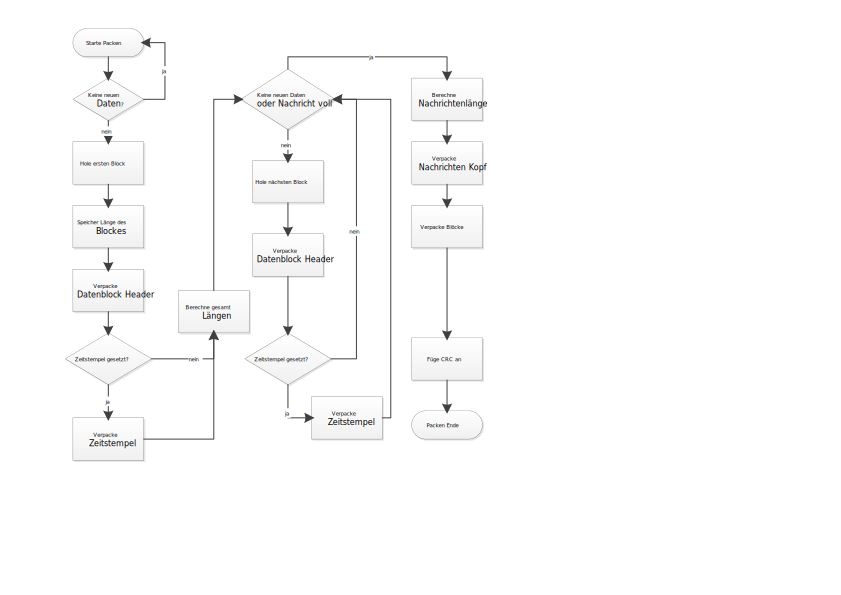
\includegraphics[scale=.5]{AlgorithmusPacketizer.jpg}
\caption{Algorithmus Packetizer}
\label{fig:AlgorithmusPacketizer}
\end{figure}

\subsection{Netzwerk}

Beschreiben der Klasse \Code{UDPSocket} und Erläuterung. Wieso wurde udp
genommen?

\subsection{StoreManager}

Während der Entwicklung des Moduls \Code{Sender} wurde eine weitere Eigenschaft
der Software gefordert.
Die Daten, welchen während des Progammablaufes erstellt und zum Versenden
gespeichert werden, sollen auch nach einem Programmabsturz oder nach einem
Stromausfall noch vorhanden sein. Weil die Klasse \Code{SmartPrioritizedQueue}
die Daten im RAM hinterlegt, wären diese verloren.
Für das Abspeichern der Daten auf die Festplatte existieren prinzipielle drei Methoden.

\begin{enumerate}
\item Jede erzeugte Variable wird direkt auf der Festplatte abgespeichert.
\item Ein Datenpacket (mehrere Variablen) wird an einer Stelle im Programm auf
einmal gespeichert.
\item Es werden Interrupts des Prozessors abgefangen, um Abstürze zu erkennen
um dann entsprechend alle wichtigen Daten zu speichern.
\end{enumerate}

Die erste Methode hat den Vorteil, dass alle Daten sofort gesichert werden und
keine verloren gehen können. Jedoch sind dafür unzählige Festplattenzugriffe
notwendig, wodurch die Laufzeit des Programms stark beeinträchtigt wird. Bei der
dritten Methode sind die Festplattenzugriffe minimal, jedoch können nur
Software- und Hardwarefehler bei der Programmabarbeitung abgefangen werden. Bei
einem Stromausfall würden trotzdem alle Daten verloren gehen. Deshalb wird
Methode Zwei verwendet. Diese stellt den besten Kompromiss aus Datensicherheit
und Performance dar. \newline
Für diese Aufgabe wurde ein Submodul entwickelt, welches die Datenblöcke auf
der Festplatte hinterlegt und bei einem Absturz neu lädt und damit die
\Code{SmartPrioritizedQueue} vorinitialisiert. Dadurch sind die Schnittstellen schon indirekt
vorgegeben, welche das Modul bereitstellen soll. Das ist eine Methode,
welche Datenblöcke auf der Festplatte speichert, eine weitere um diese zu laden
und eine dritte, mit der bereits gespeicherte Datenblöcke gelöscht werden können. 

\begin{figure}[H]
\centering
\includegraphics[scale=.5]{EinbettungStoreManager.jpg}
\caption{Integration des Submoduls \Code{StoreManager}}
\label{fig:EinbettungStoreManager}
\end{figure}

Die Einbettung des Submoduls \Code{StoreManager} in das Modul \Code{Sender} ist
in \abbildung{EinbettungStoreManager} veranschaulicht. Dazu wird der
\Code{StoreManager} parallel zur \Code{SmartPrioritizedQueue} integriert. Alle
Datenblöcke, welche in die Queue gelangen, werden ebenfalls an die
Klasse \Code{StoreManager} übergeben. Die von dem Submodul \Code{Packetizer}
gelesenen Datenblöcke werden anschliesend wieder gelöscht. Somit ist immer der
aktuelle Datenbestand der \Code{SmartPrioritizedQueue}
zusätzlich auf der Festplatte gesichert. Beim Programmstart wird in der
Initialisierungsmethode des Topmoduls überprüft, ob bereits alte Daten vorhanden
sind, welche anschliessend geladen werden. \newline
Für das Abspeichern der
Daten fehlt noch ein passendes Dateiformat, welches ein schnelle Speichern und
Lesen ermöglicht. Dazu wurden zwei Möglichkeiten gegenüber gestellt. Diese sind
in Tabelle \ref{tab:Speicherformate} aufgeführt.

\begin{longtable}{|lcc|}
\caption{Vergleich der Speicherformate} \\
\hline
\label{tab:Speicherformate}
\textbf{} & \textbf{XML-Datei} & \textbf{Binäre Datei}\\
\hline
  Menschliche Lesbarkeit      &  + & - \\
  Dateigröße      &  0 & + \\
  Geschwindigkeit &  0 & + \\
  Portabilität    &  + & - \\
\hline
\caption*{ + Gut, 0 Medium, - Schlecht }
\end{longtable}
\todo{ QUELLE???????????????????}

Der Tabelle ist zu entnehmen, dass XML auf dem ersten Blick das bessere Format
ist. Dennoch wurde eine binäre Datei verwendet, weil die beiden Schwachstellen
die Portabilität und die Lesbarkeit für einen Menschen für den konkreten
Anwendungsfall keine Bedeutung haben.
Weiterhin soll nur der Computer die Daten auf der Festplatte ablegen und
wieder lesen können Das Versenden über das Internet oder anderen
Medien besitzt damit die Portabilität keinen großen Stellenwert.
Dafür sind die beiden wichtigsten Eigenschaften, die Dateigröße und die
Geschwindigkeit, bei dem Format im Vergleich besser.
\newline
In der Datei werden die folgenden Daten aus dem Datenblock in der
aufgeführten Reihenfolge gespeichert:

\begin{itemize}
\item Datenblockheader 
\item Priorität
\item Zeitstempel
\item Content als ByteArray
\end{itemize}

Aufgrund der Tatsache, dass der Datenblockheader eine Kompression beinhaltet,
und damit die Größe der Variablen unterschiedlich sein kann, wurde für die
Variablen festgelegt, dass für jeden Wert die höchste auftretende Bitzahl
aufgerundet zu ganzen Byte verwendet wird. Dadurch wird das Laden und
Speichern stark vereinfacht. Der dabei auftretende zusätzliche
Speicherplatzbedarf kann vernachlässigt werden.
\newline 
Für die Ordnerstruktur wurde eine möglichst flache Hierachie genutzt, welche in
der obersten Stufe den Ordner Backup beinhaltet. Darin befinden sich weitere Ordner, welche
als Namen die Nummer des Datentypes beinhalten. In diesem liegen die binären
Dateien dessen Namen aus der Nummer der DOID und der Sequenznummer besteht.
Diese sind durch einen Unterstrich voneinander getrennt. Die drei Parameter
werden von der Methode remove zum Löschen einer Datei übergeben, um diese
eindeutig zu identifizieren.

\section{Modulaufbau Empfänger}

Auf der Empfängerseite sollen die ankommenden Nachrichten empfangen und geparst
werden, um an die darin enthaltenen Informationen zu gelangen. Das Empfangen
durch das Submodul \Code{UDPSocket} ist blockend. Deswegen wird der Vorgang
nebenläufig ausgeführt, damit der Programmablauf nicht behindert wird. Anschliessend wird
die Nachricht geparst und nach dem Beenden des Vorganges ein Callback
\todo{erklären was callback ist} ausgelöst.
Diese Funktion kann mittels einer Methode registriert werden, in der die
geparsten Daten weiter verarbeitet werden können. Das könnte beispielsweise die
Visualisierung dieser sein. \newline
In \abbildung{BlockdiagrammEmpfaenger} ist eine schematische
Darstellung des Moduls dargestellt. Die Implementierung wird im Folgendem näher
erläutert.

\begin{figure}[H]
\centering
\includegraphics[scale=.5]{BlockdiagrammEmpfaenger.jpg}
\caption{Übersicht des Empfängers}
\label{fig:BlockdiagrammEmpfaenger}
\end{figure}

\subsection{Parser}

Der Parser basiert auf dem in Kapitel \ref{sec:ProtokolDesign}
vorgestellten Protokoll-Design.
Anhand dieser Daten wird die empfangende Nachricht Bit für Bit analysiert
und die Informationen herrausgezogen. 
Die Klasse UDPSocket empfängt neue Daten und gibt diese an
die Klasse MessageParser weiter. Dieser parst die Nachrichtenheader. Dessen
Algorithmus ist in \abbildung{AlgorithmusMessageParser} dargestellt.
Anschließend werden die Datenblockheader geparst. Der Content wird von der
Klasse DataBlockProcessing verarbeitet.

\begin{figure}[H]
\centering
\includegraphics[scale=.5]{AlgorithmusMessageParser.jpg}
\caption{Algorithmus zum Parsen der Nachricht}
\label{fig:AlgorithmusMessageParser}
\end{figure}

Dafür wird ein Softwarekonzept namens Policy-Based-Template-Meta Programmierung
\todo{LINK buch + wiki} verwendet, damit die unterschiedlichen Datentypen der
Datenblöcke nach dem parsen wieder in einem typsicheren Format vorliegen und
einfacher verwendet werden können.
In diesem Fall werden die folgenden vier Klassen als Templateparameter Klasse
übergeben:

\begin{itemize}
\item T - Datentyp des Rückgabewertes des Parsers
\item Parser - Klasse zum Parsen des Datentypes
\item Decoder - Klasse geparsten Daten sortiert
\item C - Datentyp der als Callback zurückgegeben wird
\end{itemize}

Die beiden Parameter \Code{Parser} und \Code{Decoder} erben zusätzlich von einer
Schnittstelle. Die Klasse \Code{DataBlockProcessing} erbt
wiederum von den beiden Parametern \Code{Parser} und \Code{Decoder}.
Dadurch besteht die Möglichkeit in der Klasse auf Funktionen und
Membervariablen zugreifen zu können.
Durch dieses Vorgehen kann das Verhalten der Klasse einfach durch die
Templateparameter verändert werden. Weil der Grundalgorithmus des Parser für
die Datenblöcke für jeden Datentyp identisch ist und lediglich die Art und
Weise verändert werden muss, wie die Daten geparst oder decodiert werden müssen,
ist dieser Weg der optimalste. Durch das Konzept wurden
Redundanzen im Quellcode vermieden und weitere Datentypen lassen sich
sehr einfach hinzufügen ohne bestehenden Quellcode zu verändern. Dadurch konnten
die Grundprinzipien der objektorientierten Programmierung \todo{buch LINK}
eingehalten werden.
Der eben angesprochene Grundalgorithmus ist in Listing 
\ref{lst:PseudocodeDBParser} dargestellt, welcher für jeden Datentyp
durchlaufen wird.

\lstdefinelanguage{pseudo}{
morekeywords={if, else, for, in, remove, from, case, do, forever, to, false,
function, then, end, true, while}, sensitive=true,%
morecomment=[l]\#,%
morestring=[b]',%
}
\lstset{language=pseudo}
\lstset{commentstyle=\textit}
\lstset{literate=
{<=} {$\le$}{2} {!=} {$\neq$}{2} {=} {$\leftarrow$}{2} {==} {=}{2} {&&} {$\cap$}{2} {||} {$\cup$}{2} }
\lstinputlisting[label=lst:PseudocodeDBParser,caption=Pseudocode
des Datenblock Parsers]{Listings/PseudocodeDBParser.txt}

	\section{ChatGui}
	\label{cap:chatGui}

Dieser Abschnitt befasst sich mit der Entwicklung des \gls{GUI}. Mit dieser
wird eine nutzerfreundliche Chat-Kommunikation über die \gls{CROP}
und das \gls{ROTP} angestrebt.
Hierbei wurde auf Basis der Designregeln nach Jakob Nielsen der erste Prototyp
entwickelt.
\newline Das GUI besteht aus dem Empfangsfenster (Abbildung
\ref{fig:GUI} rechts), dem Eingabefenster (Abbildung \ref{fig:GUI}
unten links) mit einer Anzeige über bisher verschickte Nachrichten
(Abbildnug \ref{fig:GUI} oben links) sowie der Priorit{\"a}tenliste
(Abbildung \ref{fig:GUI} oben Mitte) und den Bedienelementen (Abbildung
\ref{fig:GUI} unten mitte). Die Implementierung erfolgte dabei in C++
durch die Nutzung der Qt-Bibliothek. Aufgrund der geringen Entwicklungszeit
wurde dabei von einer nutzerzentrierten \gls{GUI} Entwicklung abgesehen. Der
somit genutzte anwenderunabh{\"a}ngige Entwurf fu{\ss}t dabei auf zehn
Grunds{\"a}tzen \cite{Nielsen}.

\textbf{Regeln des \gls{GUI} Designentwurfs nach Jakob Nielsen:}

   \begin{compactenum}[I]
     \item \textit{Nutzung einfacher und nat{\"u}rlicher Dialoge}
     \item \textit{Verwendung der Nutzersprache}
     \item \textit{Minimierung der Ged{\"a}chtnislast des Nutzers}
     \item \textit{Nutzung konsistenter Formulierungen}
     \item \textit{Dem Nutzer stets Feedback geben}
     \item \textit{Klar markierte Navigationsm{\"o}glichkeiten anbieten}
     \item \textit{Dem Nutzer Shortcuts anbieten}
     \item \textit{Lieferung genauer Fehlermeldungen}
     \item \textit{Vermeidung vermeidbarer Fehler}
     \item \textit{Bereitstellen einer Hilfe und Dokumentation}
   \end{compactenum}
   \label{Nielsen}

Je nach Komplexit{\"a}t des vorliegenden Projekts gilt es, einzelne Punkte
hierbei eventuell schwerer zu gewichten als andere. So steigt z.B. bei
zunehmender Komplexit{\"a}t des \gls{GUI} die Wichtigkeit einer ausf{\"u}hrlichen
Hilfe und Dokumentation. Da die Komplexit{\"a}t des \gls{GUI} im Szenario der
Projektarbeit {\"u}berschaubar ist, wurde auf eine Hilfefunktion verzichtet
und diese durch eine ausf{\"u}hrliche Dokumentation ersetzt (Regel zehn nach
Nielsen).

\begin{figure}[H]
\centering
\includegraphics[width=\textwidth]{GUI_1.pdf}
\caption{Grafische Benutzeroberfläche (MarsChat)}
\label{fig:GUI}
\end{figure}

Die Abbildung \ref{fig:GUI} zeigt das \gls{GUI} im {\"U}berblick. Die auf den
ersten Blick ungew{\"o}hnlich anmutende (getrennte) Anordnung von Sende- und
Empfangsfenster ist das Resultat der stark verz{\"o}gerten Kommunikation. Da
Satzteile unterschiedliche Priorit{\"a}ten aufweisen k{\"o}nnen und somit die
{\"U}bertragung einer Nachricht {\"u}ber einen l{\"a}ngeren Zeitraum erfolgen
kann, ist eine gew{\"o}hnliche Chatoberfl{\"a}che ungeeignet. In der getrennten
Anordnung kann die mit Verz{\"o}gerung empfangene Nachricht im rechten Teil des
\gls{GUI} aufgebaut werden, w{\"a}hrend im linken Teil weiterhin Nachrichten
verschickt werden k{\"o}nnen\footnote{F{\"u}r die Zukunft ist eine weitere Verbesserung dieses
Verhaltens vorgesehen, sodass vollst{\"a}ndig empfangene Nachrichten im
Sendefenster in die Kommunikation chronologisch eingeordnet werden.}. \newline
\newline Die grundlegende Funktionalit{\"a}t des \gls{GUI} entspricht der eines
{\"u}blichen Chat-Programms, welches Eingaben {\"u}ber ein Textfeld erm{\"o}glicht und diese
nach Best{\"a}tigung versendet. Die Eingabe erfolgt {\"u}ber das Textfeld im
linken unteren Bereich des \gls{GUI}. Nach erfolgter Eingabe kann die Nachricht
durch Dr{\"u}cken des Senden Buttons oder per Shortcut (Regel sieben nach
Nielsen) verschickt werden.
Sollte dies geschehen, ohne zuvor einem Wort, Satzteil oder Satz eine
Priorit{\"a}t zuzuordnen, wird der Eingabe die Standardpriorit{\"a}t Null
zugeordnet. F{\"u}r den Fall, dass zuvor eine Priorisierung erfolgen soll,
besteht die M{\"o}glichkeit, dies mit Hilfe der in der Mitte (unten)
befindlichen Steuerelemente zu tun. Diese sind klar und eindeutig bezeichnet und nach
Zusammengeh{\"o}rigkeit angeordnet (Regel sechs nach Nielsen). Fehleingaben wie
beispielsweise das Versenden leerer Nachrichten werden nach Regel neun durch das
\gls{GUI} verhindert.

\begin{figure}[H]
\centering
\includegraphics[width=8cm]{Msg_2.pdf}
\caption{Beispiel einer Information}
\label{fig:Msg2}
\end{figure}

\begin{figure}[H]
\centering
\includegraphics[width=8cm]{Msg_3.pdf}
\caption{Beispiel einer Warnung}
\label{fig:Msg3}
\end{figure}

Der User erh{\"a}lt dabei immer Feedback in Form von
Informationsdialogen oder Warnhinweisen (siehe Abbildung \ref{fig:Msg2} und
Abbildung
\ref{fig:Msg3}). Zudem gibt es Feedback in Form von optionalen Meldungen, die
der User je nach Bedarf deaktivieren kann, um so f{\"u}r eine Zeitersparnis zu
sorgen (siehe Abbildung \ref{fig:Msg1}). Somit erfahren auch Regel f{\"u}nf und
acht nach Nielsen eine Umsetzung.

\begin{figure}[H]
\centering
\includegraphics[width=8cm]{Msg_1.pdf}
\caption{Beispiel einer optionalen Mitteilung}
\label{fig:Msg1}
\end{figure}

Auch die Formulierungen der Dialoge und Bedienelemente unterliegen dabei den
geforderten Regularien (Regeln eins, zwei, vier nach Nielsen). Die im mittleren
oberen Bereich des \gls{GUI} angeordnete Liste beinhaltet die vom User
vergebenen Priorit{\"a}ten. Da die bereits priorisierten Textpassagen zudem farblich
markiert werden, muss der User sich nicht merken, welche Bereiche er bereits
priorisiert hat. Es erfolgt somit eine Minimierung der Ged{\"a}chtnislast des
Users (Regel drei nach Nielsen).


\chapter{Protokoll-Analyse}
	\label{cap:protokollAnalyse}
Zur fundierten Aussage über die Funktionsfähigkeit und -tragweite des CROP wurde
dieses hinsichtlich unterschiedlicher Aspekte untersucht. Dazu gehört neben der
Laufzeit und Paketgröße auch der Overhead. Unter verschiedenen Einstellungen
wurden mehrere Messreihen aufgenommen, welche im Folgenden näher vorgestellt und
diskutiert werden.

	\section{Overhead}
		Wie bereits im Kapitel \ref{sec:ProtokolDesign} erläutert, existiert neben den
eigentlichen Daten der Header. Die zusätzliche Größe, um die sich die
zu versendende Nachricht dadurch erhöht, heißt Overhead. Die Berechnung und
Bedeutung dessen wird im Folgenden beschrieben.

Ausgehend vom Aufbau einer Nachricht (siehe Abbildung
\ref{fig:uebersichtdatenaufschluesselung_text}) sind bei der Berechnung des
Overhead zwei Header zu betrachten. Einerseits ist dies der allgemeine Header der
Nachricht und zum anderen trägt jeder einzelne Datenblock
mit einem eigenen Header zum Overhead bei. Dies kann durch die Formel
\ref{eq:overhead} ausgedrückt werden.

\begin{equation}
	Overhead = Overhead_{Nachricht} + n * Overhead_{Datenblock}
	\label{eq:overhead}
\end{equation}

Dabei variiert die Größe des Nachrichtenheaders je nach gewähltem
Übertragungsprotokoll (Formel \ref{eq:overheadMessage}). In dem Protokoll,
welches in dieser Arbeit vorgestellt wird, ist dies das IPv6. Das IPv6
reserviert $32$ Byte im Header. Damit ergeben sich für diesen speziellen
Fall $37$ Byte für den Nachrichtenheader. Ein Datenblockheader besteht immer
konstant aus $9$ Byte.
Die angedeutete Kompressionseinstellung findet in dieser Arbeit noch
keine Berücksichtigung.

\begin{equation}
	Overhead_{Nachricht} = 5 Byte + Address_{Source} + Address_{Destination}
	\label{eq:overheadMessage}
\end{equation}

Aus der Formel \ref{eq:overhead} ist zu erkennen, dass der Overhead
stetig mit der Anzahl an gleichzeitig zu verschickenden Datenblöcken ($n$)
steigt. Einzig der Nachrichtenoverhead hat für große $n$ nur noch eine
geringe Auswirkung. Somit ist ein Versenden einer Nachricht mit vielen Daten
gleichzeitig sinnvoller, um überflüssigen Overhead zu vermeiden. Dieser
Effekt wird mit Formel \ref{eq:overheadRatio} noch einmal verdeutlicht. Diese
gibt das Verhältnis der Größe von Overhead zur gesamten Nachricht an und
ermöglicht eine prozentuale Aussage.

\begin{eqnarray} 
	overhead_{ratio} & = & \frac{Overhead}{Nachricht_{gesamt}}\\
	overhead_{ratio} & = & \frac{Overhead_{Nachricht} + n * Overhead_{Datenblock}}{Overhead_{Nachricht} + n * (Overhead_{Datenblock} + Content)}\\
	overhead_{ratio} & = & \frac{Overhead}{Overhead + n * Content}
	\label{eq:overheadRatio}
\end{eqnarray}

Der vorgestellte Sachverhalt soll im Folgenden an einem Beispiel
verdeutlicht werden. Hierzu wird wie ein Text mit $5.000.000$ Byte herangezogen.
Zunächst soll der Text ohne relevante Bereiche übertragen werden. Das heißt,
dass für den kompletten Inhalt nur ein einziger Datenblock benötig wird. Damit
ergibt sich, ausgehend von Formel \ref{eq:overheadRatio} folgendes Bild für den
Overhead ($Overhead_{worp}$).

% \begin{eqnarray} 
% 	Overhead_{worp} & = & Overhead_{Nachricht} + n * Overhead_{Datenblock} \\
% 	Overhead_{worp} & = & Overhead_{Nachricht} + Overhead_{Datenblock} \\
% 	Overhead_{worp} & = & 37 Byte + 9 Byte \\
% 	Overhead_{worp} & = & 46 Byte
% 	\label{eq:overheadRatio_worp}
% \end{eqnarray}

\begin{eqnarray} 
	Overhead_{worp} & = & \frac{Overhead}{Nachricht_{gesamt}}\\
	Overhead_{worp} & = & \frac{Overhead_{Nachricht} + n * Overhead_{Datenblock}}{Overhead_{Nachricht} + n * (Overhead_{Datenblock} + Content)}\\
	Overhead_{worp} & = & \frac{46 Byte}{46 Byte + 5.000.000 Byte} \\
	Overhead_{worp} & = & 0,92 \cdot 10^{-3} \%
	\label{eq:overheadRatio_worp}
\end{eqnarray}

Der selbe Text wird jetzt mit $50$ wichtigen Fragmenten versehen. Damit ändert
sich der Overhead ($Overhead_{wrp}$) wie in Formel \ref{eq:overheadRatio_wrp}
dargestellt ab.

% \begin{eqnarray} 
% 	Overhead_{wrp} & = & Overhead_{Nachricht} + n * Overhead_{Datenblock} \\
% 	Overhead_{wrp} & = & Overhead_{Nachricht} + 50 * Overhead_{Datenblock} \\
% 	Overhead_{wrp} & = & 37 Byte + 50 * 9 Byte \\
% 	Overhead_{wrp} & = & 487 Byte
% 	\label{eq:overheadRatio_wrp}
% \end{eqnarray}

\begin{eqnarray} 
	Overhead_{wrp} & = & \frac{Overhead}{Nachricht_{gesamt}}\\
	Overhead_{wrp} & = & \frac{Overhead_{Nachricht} + n * Overhead_{Datenblock}}{Overhead_{Nachricht} + n * (Overhead_{Datenblock} + Content)}\\
	Overhead_{wrp} & = & \frac{487 Byte}{487 Byte + 5.000.000 Byte} \\
	Overhead_{wrp} & = & 9,7 \cdot 10^{-3} \%
	\label{eq:overheadRatio_wrp}
\end{eqnarray}

Eine Gegenüberstellung der beiden Werte (Formel \ref{eq:overheadRatio_wrp_worp})
zeigt, dass sich das Einfügen von relevanten Bereichen nachteilig auf den
Overhead auswirkt. Je mehr dieser Fragmente vorhanden sind, desto größer wird
die zu übertragende Nachricht. Somit ist beim Versand eines Texten mit $50$
relevanten Bereichen mit einem fast elf mal so hohem Overhead zu rechnen.

\begin{eqnarray} 
	\frac{ Overhead_{wrp} }{ Overhead_{worp} } & = & \frac{9,7 \cdot 10^{-3} \%}{0,92 \cdot 10^{-3} \%} \\
	\frac{ Overhead_{wrp} }{ Overhead_{worp} } & = & 10,5 \\ 
	Overhead_{wrp} & = & 10,5 \cdot Overhead_{worp}
	\label{eq:overheadRatio_wrp_worp}
\end{eqnarray}

Es ist zu sehen, dass der 
	\section{Messreihen}
		\label{subCap:Messreihen}

Die Messungen wurden mit einem Notebook aufgenommen, welches
folgende Hardwarekonfigurationen besitzt.

\textit{
	LENOVO Thinkpad t410 Modell 2522-w29 \newline
	\textbf{Prozessor}: Intel Core i5 520M (2 Kerne mit Hyperthreading $\stackrel{\wedge}=$ 4 Threads)\\
	\textbf{Arbeitsspeicher}: 4 GB DDR3	
	}

Da eine ähnliche Hardware bei einer Verwendung des Protokolls auf dem Mars
weniger zu erwarten ist, sind die Größenordnungen der nachfolgenden Ergebnisse
nur ein Richtwert. Für die folgenden Betrachtungen sind die Beziehungen und
Entwicklungen der einzelnen Werte zueinander wichtig, welche mit schwächerer
Hardware nahezu identisch sind.

Das Protokoll wird grundlegend mit zwei verschiedenen
Compilereinstellungen getestet. Zum einen die Geschwindigkeits- (\glqq O$2$
\grqq) und zum Anderen die Quellcodegrößenoptimierung (\glqq Os \grqq). Dabei
wurde untersucht, wie lange das Protokoll für die Verarbeitung von Texten
verschiedener Größe benötigt, die keine relevanten Bereiche besitzen. Dafür
wurden Dateien mit verschiedenen Größen von $2$ Bytes bis $10$ Millionen Bytes 
angelegt, durch das Programm eingelesen und der Schnittstelle des Protokolls
übergeben. In diesem Fall ist keine Vorpriorisierung notwendig und die Datei
kann sukzessive in maximale Datenblockgrößen zerlegt werden.
Im Vergleich dazu ist eine Messreihen mit unterschiedlich vielen relevanten
Bereichen für einen Text mit der Größe von $5.000.000$ Byte aufgenommen
worden.
Durch das Anfallen von zusätzlichen Berechnungen die zum Zerteilen 
des Textes notwendig sind, ist zu erwarten, dass die Laufzeit gegenüber
ersterer Betrachtung ansteigt.

Die eben vorgestellten Messungen wurden auf zwei verschiedenen Wegen
aufgenommen. Diese unterscheiden sich dahingehend, dass das Modul vor dem Erhalt
neuer Daten gelöscht und anschließend neu erstellt wurde. Somit sind alle
Datenstrukturen bei jeden Messdurchgang leer, wodurch vorallem die Komplexität
der Einsortierung in die priorisierende \gls{FIFO} verringert wurde. Für den
zweiten Fall wurden die Daten alle nacheinander verschickt, um ein realistischeres
Szenario darzustellen zu können.

Für einen aussagekräftigeren Wert und um potentielle Messungenauigkeiten zu
kompensieren, wurde die Messung für jede Einstellung $10$ Mal wiederholt und der
Mittelwert gebildet. Die Messreihen sind zur besseren Übersicht im
Anhang dargestellt (\ref{sec:messtabellen}).
	\section{Ergebnisse und Diskussion}
		Die Abbildung \ref{fig:diagrammInitial_worp} zeigt grafisch die Ergebnisse der
Messreihen für den initialen Durchlauf ohne relevante Bereiche. Dabei ist die
Laufzeit in $µs$ über die Textgröße in Byte logarithmisch aufgetragen. Für
relativ kleine Textgrößen hat die Geschwindigkeitsoptimierung noch keine großen
Einfluss. Erst bei einer Größe von $5.000.000$ ($99$ µs) oder
$10.000.000$ ($122$ µs) Byte ist der erwartete Geschwindigkeitsprofit zu
verzeichnen.

\begin{figure}[H]
	\centering
	\includegraphics[width=\textwidth]{DiagrammInitial_worp.pdf}
	\label{fig:diagrammInitial_worp}
	\caption{Messung-Initial ohne relevante Bereiche}
\end{figure}

Der Nachteil gegenüber der Quellcodegrößenoptimierung liegt darin, dass
mehr Speicherplatz in Anspruch genommen wird, wodurch der
Geschwindigkeitsvorteil erreicht werden kann.
Die Wahl der jeweiligen Optmierungsmöglichkeit ist situationsabhängig. Auf dem
Mars stehen weniger Speicherressourcen zur Verfügung, wodurch eine
Geschwindigkeitsoptimierung weniger sinnvoll erscheint. Die gleichen
Betrachtungen ergeben sich für alle anderen Messreihen (Abbildung
\ref{fig:diagrammInitial_wrp}, \ref{fig:diagrammNormal_worp}, \ref{fig:diagrammNormal_wrp}). 

In Abbildung \ref{fig:diagrammInitial_wrp} ist die Laufzeit bezüglich
verschiedener Anzahlen relevanter Bereiche dargestellt. Die Textgröße bleibt
dabei stetig bei $5.000.000$ Byte. Damit ist ein Vergleich der Werte mit den
durchschnittlichen Werten der gleichen Textgröße aus Abbildung
\ref{fig:diagrammInitial_worp} möglich. Für nur wenige relevante Bereiche
unterscheiden sich die Werte maginal. Steigt die Anzahl, nimmt die Laufzeit
jedoch exponentiell zu (siehe Abbildung \ref{fig:diagrammInitial}) und bewegen
sich im Millisekunden-Bereich. Dies Bedeutet, dass die Implementierung noch
nicht für die Verwendung von einer sehr große Anzahl an relevanten Bereichen
optimiert wurde. Im Kapitel \ref{sec:Anwendungsszenarien} wurden bereits
mögliche Anwendungsszenarien betrachtet, welche ebenso mit wenigen relevanten
Bereichen auskommen. Dadurch ist eine Optimierung an dieser Stelle vorerst
nebensächlich.

\begin{figure}[H]
	\centering
	\includegraphics[width=\textwidth]{DiagrammInitial.pdf}
	\label{fig:diagrammInitial}
	\caption{Messung-Initial}
\end{figure}

\todo{ bild einfügen wobei man darauf wohl nicht viel erkennt?}
Die Messung ist in Abbildung MUH dargestellt, bei der nacheinander
unterschiedliche Datengrößen verarbeitet werden und das Modul nicht neu erstellt
wurde. Hierbei ist zu erkennen, dass die Dauer immer grösser wird
je mehr Daten schon bearbeitet wurden. Eine genauere Analyse zeigt, dass die
priorisierenden \gls{FIFO} der Flaschenhals ist. Bei diesen Testdurchlauf
wurden insgesamt $41.400$ Datenblöcke aus $548$ MB bewältigt. Dabei lagen alle
Datenblöcke gleichzeitig in der \gls{FIFO}, wodurch das Einsortieren neuer
Blöcke sehr viel Rechenleistung in Anspruch nimmt. Gleichzeitig werden diese
Daten im Arbeitsspeicher und auf der Festplatte gespeichert. Hierbei gilt zu
untersuchen, ob diese Form der Datensicherung bei einem Rover auf dem
Mars praktikabel ist, da dieser über sehr begrenzte Speicherressourcen verfügt.
Alternativ müssen neue Methoden gefunden werden den Speicherverbrauch
einzuschränken. So besteht die Möglichkeit die Daten nur auf der Festplatte
zu speichern und in der \gls{FIFO} die Indizies zu diesen zu hinterlegen,
wodurch der Speicherverbrauch im Arbeitsspeicher stark reduziert werden kann.
Allerdings ist diese Methode bei sehr vielen Daten nicht optimal, welche sich
bei sehr langen Zeiträumen in denen nicht gesendet werden kann ansammeln.
Eine bessere Möglichkeit wäre anhand einer \gls{TTL} (siehe Kapitel
\ref{sec:Vorueberlegung}) unrelevante Daten nur sehr kurzfristig vorzuhalten, damit mehr Raum für Daten
von hoher Relevanz ist.


\chapter{Zusammenfassung und Ausblick}
	% Zusammenfassung

Für die interplanetare Kommunikation stehen besondere Aspekte, wie Latenz,
Bandbreite oder der lokale Speicher im Vordergrund. Dazu ist ein besonderes
Kommunikationsprotokoll notwendig. Für dieses Protokoll existiert
bereits ein Konzept \cite{Daher}, welches im Rahmen dieser Arbeit
teilweise verfeinert, implementiert und bewertet wurde.

Das Kapitel \ref{cap:grundlagen} beschäftigte sich
mit den momentanen Stand der Technik sowie den Grundlagen zur Einordnung der
Thematik. Dabei wurde eine Übersicht über die grundlegenden Begriffe im
Bereich der Kommunikation gegeben. Weiterhin wurde die Bedeutung und
Auswirkung eines geringen Zeitslots für die Kommunikation zwischen Mars und Erde
verdeutlicht.\newline
Einen umfassenden Überblick über aktuelle Technologien, welche auf heutigen
Marsmissionen eingesetzt werden, werden in Kapitel \ref{cap:standDerTechnik}
dargelegt.
Dabei wird neben der verbauten Technik der Marsrover auch bisher verwendete
Kommunikationsprotokolle vorgestellt.

In Kapitel \ref{cap:konzept} wurden weitere Ansätze und Ideen für das Konzept
\gls{CRODT}/\gls{CROP} vorgestellt dieses zu verfeinern. Dabei wurde die
Möglichkeit der Verwendung einer \gls{TTL}, einer Datenkompression und einer
Prüfsumme diskutiert. Für die Realisierung wurde ein Protokoll-Design
entwickelt. Darin wurden die optimale Größen und Anordnungen der Daten erörtert,
um ein Ver- und Entpacken unterschiedlicher Datenformate auf beiden Seiten der
Kommunikation zu ermöglichen.
Schlussendlich wurde anhand von Anwendungsszenarien die Schnittstellen der
Module abgeleitet, welche in der Realisierung verwendet wurden.

Der softwaretechnische Aufbau und die Realisierung des Konzepte
wurde in Kapitel \ref{cap:implementierung} detailliert beschrieben. Dabei wurde
jeweils ein Modul zum Empfangen und Senden implementiert.
Dabei wurden auch Verbindungsabbrüche und Systemabstürze berücksichtigt, worauf
das Modul \Code{StoreManager} entwickelt wurde. Dieses ist in der Lage nach
einem Fehler den vorherigen Zustand wiederherzustellen.
Weiterhin wurde eine Kommunikationsumgebung in Form eines ChatGui entwickelt.
Unter Verwendung des \gls{ROTP} können hier Prioritäten vom Benutzer selbst
festgelegt und vom CROP verarbeitet werden. Damit steht eine Beispielanwendung
zur Verfügung, mit dessen Hilfe sich unter anderem die Effizienz von
M$2$M-Kommunikation des \gls{CROP}-Protokolls durchführen läßt.

Abschließend wurde im Kapitel \ref{cap:protokollAnalyse} das Protokoll
hinsichtlich Overhead, Laufzeit und Speicherbedarf analysiert und ausgewertet.
Dabei kamen zwei verschiedene Compilereinstellungen zum Einsatz, die entweder
die Größe des Quellcodes oder die Laufzeit des Programms beeinflussen. Die
Ergebnisse der Analyse zeigten wie wichtig eine sinnvolle Priorisierung durch
die CROP ist und wie stark der Overhead und die Laufzeit von dieser abhängen.

% Ausblick
Das in dieser Arbeit umgesetzte Protokoll bietet eine solide
Grundlage zur relevanzorientierten Übertragung. Jedoch besteht noch Raum
für Erweiterungen und Optimierungen.

So ist z.B. eine Optimierung der implementierten Algorithmen sinnvoll.
Der erste Anhaltspunkt ist das Submodul \Code{StoreManager}.
Die Zugriffe auf ein Speichermedium während des kontinuierlichen Speicherns und
Ladens der Daten sind sehr langsam und bremsen das gesamte Modul. Eine
Möglichkeit, dies zu verbessern, wäre, das Modul in einem extra Prozess
auszuf{\"u}hren. Dann wären die Zugriffe unabhängig vom eigentlichen
Programmablauf. Ein weiterer Ansatzpunkt ist die Datenstruktur
\Code{SmartPrioritizedQueue}. Für diese muss eine effiziente Möglichkeit
gefunden werden, Datenblöcke schnell einzusortieren, zu löschen und Bl{\"o}cke
bestimmter Größe zu finden.
Die angedachte Kompressionseinstellung aus Kapitel \ref{sec:ProtokolDesign}
findet beispielsweise im \Code{StoreManager} schon Berücksichtigung, wurde aber
noch nicht vollständig implementiert. Dadurch kann in Zukunft für viele kleine
Datenblöcke weiterer Overhead eingespart werden.

Das Protokoll ist aufgrund seiner Flexibilität auf eine Vielzahl an Datentypen
anwendbar. Die Handhabung vieler Daten eines Datentyps zur selben Zeit kann
in Form von parallel ablaufenden Prozessen zur Geschwindigkeitsoptimierung
beitragen. Um andere Datentypen im Protokoll zu verwenden, sollte eine
Schnittstelle zum Laden von Plugins implementiert werden. Damit besteht dann die
Möglichkeit, dem Protokoll Algorithmen hinzuzufügen, wodurch
übliche Datenformate wie docx oder bmp verarbeitet werden können.

Das ebenfalls im Rahmen dieser Arbeit entwickelte ChatGui in Kapitel
\ref{cap:chatGui} hinsichtlich des Zusammenführens der einzelnen Textfragmente
zu optimiert. Sinnvoll wäre hier eine Anzeige über die ablaufende Zeitdauer,
nach welcher ein versendetes Paket den Empfänger erreicht.

Um das entwickelte Modul in Serverumgebungen zu integrieren, muss ein Programm
entwickelt werden, welches in der Lage ist, dieses als Webservice zu starten.
Dadurch können schon bestehende Benutzeroberflächen das Protokoll nutzen.



%\bibliographyWebverzeichnis{Webverzeichnis}
%\bibliographystyleWebverzeichnis{plain}
%\nociteWebverzeichnis{*}

% Literaturverzeichnis ---------------------------------------------------------
%   Das Literaturverzeichnis wird aus der BibTeX-Datenbank "Referenzen.bib"
%   erstellt.
% ------------------------------------------------------------------------------
\renewcommand{\refname}{Literatur- und Webverzeichnis}
\RaggedRight
\bibliography{Referenzen} % Aufruf: bibtex BLA-Arbeit
\bibliographystyle{natdin} % DIN-Stil des Literaturverzeichnisses

Eidesstattliche Erklärung

\vspace{2cm}

Hiermit erkläre ich an Eides statt, dass ich die vorliegende Arbeit
selbstständig und ohne Benutzung anderer als der angegebenen Hilfsmittel
angefertigt habe. Die aus den Quellen direkt oder indirekt übernommenen
Gedanken sind als solche kenntlich gemacht.

\vspace{1cm}

Die Arbeit hat mit gleichem bzw. in wesentlichen Teilen gleichem Inhalt noch
keiner anderen Prüfungsbehörde vorgelegen.

\vspace{4cm}

Ort, Datum \hspace{5cm} Unterschrift % Selbständigkeitserklärung

% Anhang -----------------------------------------------------------------------
%   Die Inhalte des Anhangs werden analog zu den Kapiteln inkludiert.
%   Dies geschieht in der Datei "Anhang.tex".
% ------------------------------------------------------------------------------
\begin{appendix}
    \clearpage
    \pagenumbering{roman}
    \chapter{Anhang}
    \label{sec:Anhang}
    % Rand der Aufzählungen in Tabellen anpassen
    \setdefaultleftmargin{1em}{}{}{}{}{}
    Nachfolgend wird eine Anleitung dargestellt, um die in
dieser Arbeit verwendeten Tools einzurichten, womit der erstellte
Quellcode kompiliert werden kann. Weiterhin wird ein Anwendungsbeispiel
gegeben, welches die statische Bibliothek nutzt. Dazu werden die notwendigen
Header-Dateien aktualisiert und in das Beispiel eingebunden.

\section{Vorbereitungen}

Als Betriebssystem wurde Ubuntu 12.4 verwendet. In diesem m{\"u}ssen
{\"u}ber den Packetmanager zuerst folgenden Programme und Bibliotheken installiert
werden, wenn diese noch nicht vorhanden sind.

\begin{itemize}
\item "`libboost-all-dev"' (ab Version 1.48.0.2) 
\item "`libqt4-dev"' (ab Version 4.8)
\item "`gcc"' (ab Version 4.6.3)
\item "`build-essential"'
\end{itemize}

Im n{\"a}chsten Schritt wird die Eclipse IDE for C/C++
Developers\footnote{http://www.eclipse.org/downloads/packages/release/helios/sr2}
heruntergeladen und eingerichtet. F{\"u}r dieses wurden die folgenden Plugins installiert:

\begin{itemize}
\item EGit\footnote{http://download.eclipse.org/egit/updates-nightly}
\item QT
% \footnote{http://blog.qt.digia.com/2007/07/11/develop-qt-applications-in-eclipse/}
alternativ QT Creator
\end{itemize}

Das Installieren von Plugins unter Eclipse erfolgt {\"u}ber \Code{Help $\rightarrow$
Install New Software\ldots} durch die Eingabe der in Fu{\ss}noten stehenden
Internetadresse. Zum kompilieren der grafischen Benutzeroberfl{\"a}che sollte die
QT eigene Entwicklungsumgebung QT Creator \todo{link zuf{\"u}gen} genutzt werden.
Das QT-Plugin f{\"u}r Eclipse ist auf der Webseite derzeit nicht herunterladbar.

\section{Git}

Als Erstes sollte eine SSH verbindung zum Git-Repository eingerichtet werden.
Dazu sei auf die Anleitung von Git verwiesen
\todo{https://help.github.com/articles/generating-ssh-keys}. Als n{\"a}chstes k{\"o}nnen
die Quelldateien unter Eclipse heruntergeladen werden. Dazu wird im Eclipse die
Ansicht zum Git-Repository gewechselt. Dies erfolgt mit \Code{Window
$\rightarrow$ Open Perspective $\rightarrow$ Other\ldots $\rightarrow$ Git
Reposity Exploring}. In der neuen Ansicht das Herunterladen durch anklicken des
Icons "`Clone a Git Repository and add the clone to this view"'. Im sich {\"o}ffnenden
Assistenten m{\"u}ssen unter URI die SSH-Daten
\Code{ssh://git@github.com/Helferlein/CAVLOD.git} eingetragen und
beim letzten Fenster sollte ein Pfad angegeben werde, welcher
unabh{\"a}ngig des Workspaces von Eclipse ist.\newline
Danach wird die Ansicht auf \Code{Window
$\rightarrow$ Open Perspective $\rightarrow$ Other\ldots $\rightarrow$ C/C++}
zur{\"u}ckgesetzt. Unter \Code{File $\rightarrow$ Import\ldots Git $\rightarrow$
Projects from Git $\rightarrow$ local} kann das entsprechende Projekt von Git
in die Eclipse-Projektumgebung importiert werden. Zum Kompilieren kann
mit Rechtsklick auf den Projektname und Auswahl des Buildes (\Code{Build Configurations
$\rightarrow$ Set Active}) das Programm erstellt werden. Hierf{\"u}r existieren
drei Auswahlm{\"o}glichkeiten:

\begin{enumerate}
\item \Code{client} bezeichnet die Testumgebung, welches
Daten an den Sender {\"u}bergibt, der diese verarbeitet und {\"u}ber eine UDP-Schnitttelle ausgibt. 
\item \Code{server} bezeichnet die Testumgebung, welche die
Daten vom Client empf{\"a}ngt und ausgibt.
\item \Code{statLib} erstellt eine statische Bibliotheke zum weiterverwenden der
Module in einem anderen Projekt.
\end{enumerate}

Der Kompiliervorgang kann durch Rechtsklick auf den Projektname und ausw{\"a}hlen
von \Code{Build Project} gestartet werden.

\section{Beispiel}

Nach erfolgreicher erstellen der Bibliothek m{\"u}ssen die folgenden Dateien
im Pfad \Code{Crodt/include/} der statischen Bibliotheke aktualisiert werden,
wenn diese ge{\"a}ndert wurden. Ebenso wie die erstellte Datei
\Code{Crodt/lib/libcrodt.a}.

\begin{itemize}
\item \Code{src/DataManagement/CrodtIO.h} 
\item \Code{src/Modules/ReceiverModule.h}
\item \Code{src/Modules/ReceiverModuleIF.h}
\item \Code{src/Modules/SenderModule.h}
\item \Code{src/Modules/SenderModuleIF.h}
\end{itemize}

Zur Verwendung sind zwei Beispielquellcodes in Listing
\ref{lst:BeispielcodeSender} und \ref{lst:BeispielcodeReceiver} dargestellt. Der
erste erstellt ein Sendermodul und {\"u}bergibt diesen die passenden Daten, die
gesendet werden sollen. Beim Zweiten wird ein Empfangsmodul erstellt. In diesem
wird ein Callback registriert, welches die empfangenen Daten auf der Konsole
ausgibt. Dabei sei zu beachten, dass in beiden die Header-Datei \Code{crodt.h}
inkludiert werden muss.

\newpage

\lstset{language=C++}
\lstinputlisting[label=lst:BeispielcodeSender, caption=Anwendungsbeispiel:
Sender]{Listings/BeispielcodeSender.cpp}


\lstset{language=C++}
\lstinputlisting[label=lst:BeispielcodeReceiver, caption=Anwendungsbeispiel:
Receiver]{Listings/BeispielcodeReceiver.cpp}

\end{appendix}

% Index ------------------------------------------------------------------------
%   Zum Erstellen eines Index, die folgende Zeile auskommentieren.
% ------------------------------------------------------------------------------
%\printindex

\end{document}
